%----------------------------------------------------------------------------
\chapter{Overview of the Approach} \label{overviewoftheapproach}
%----------------------------------------------------------------------------
In this chapter, the various aspects of the proposed approach are detailed. In Section \ref{sec_methodology}, the application of this methodology is presented from the users' point of view: how to use the interactive automata learning framework -- also called \textit{Interactive Learning Entity} or \textit{ILE} - and how they can utilize it to design reactive systems in a declarative way. Then, in Section \ref{sec_architecture}, the applied software architecture, software components, algorithms and data structures are presented: first, the components concerned with the automata learning algorithm, then those responsible for its interaction with the oracle component, then the possible interactions of the oracle with the engineer.
%----------------------------------------------------------------------------
\section{Overview of the Methodology} \label{sec_methodology}
%----------------------------------------------------------------------------
\begin{figure}[!ht] 
	\centering
	
	%\fbox{
		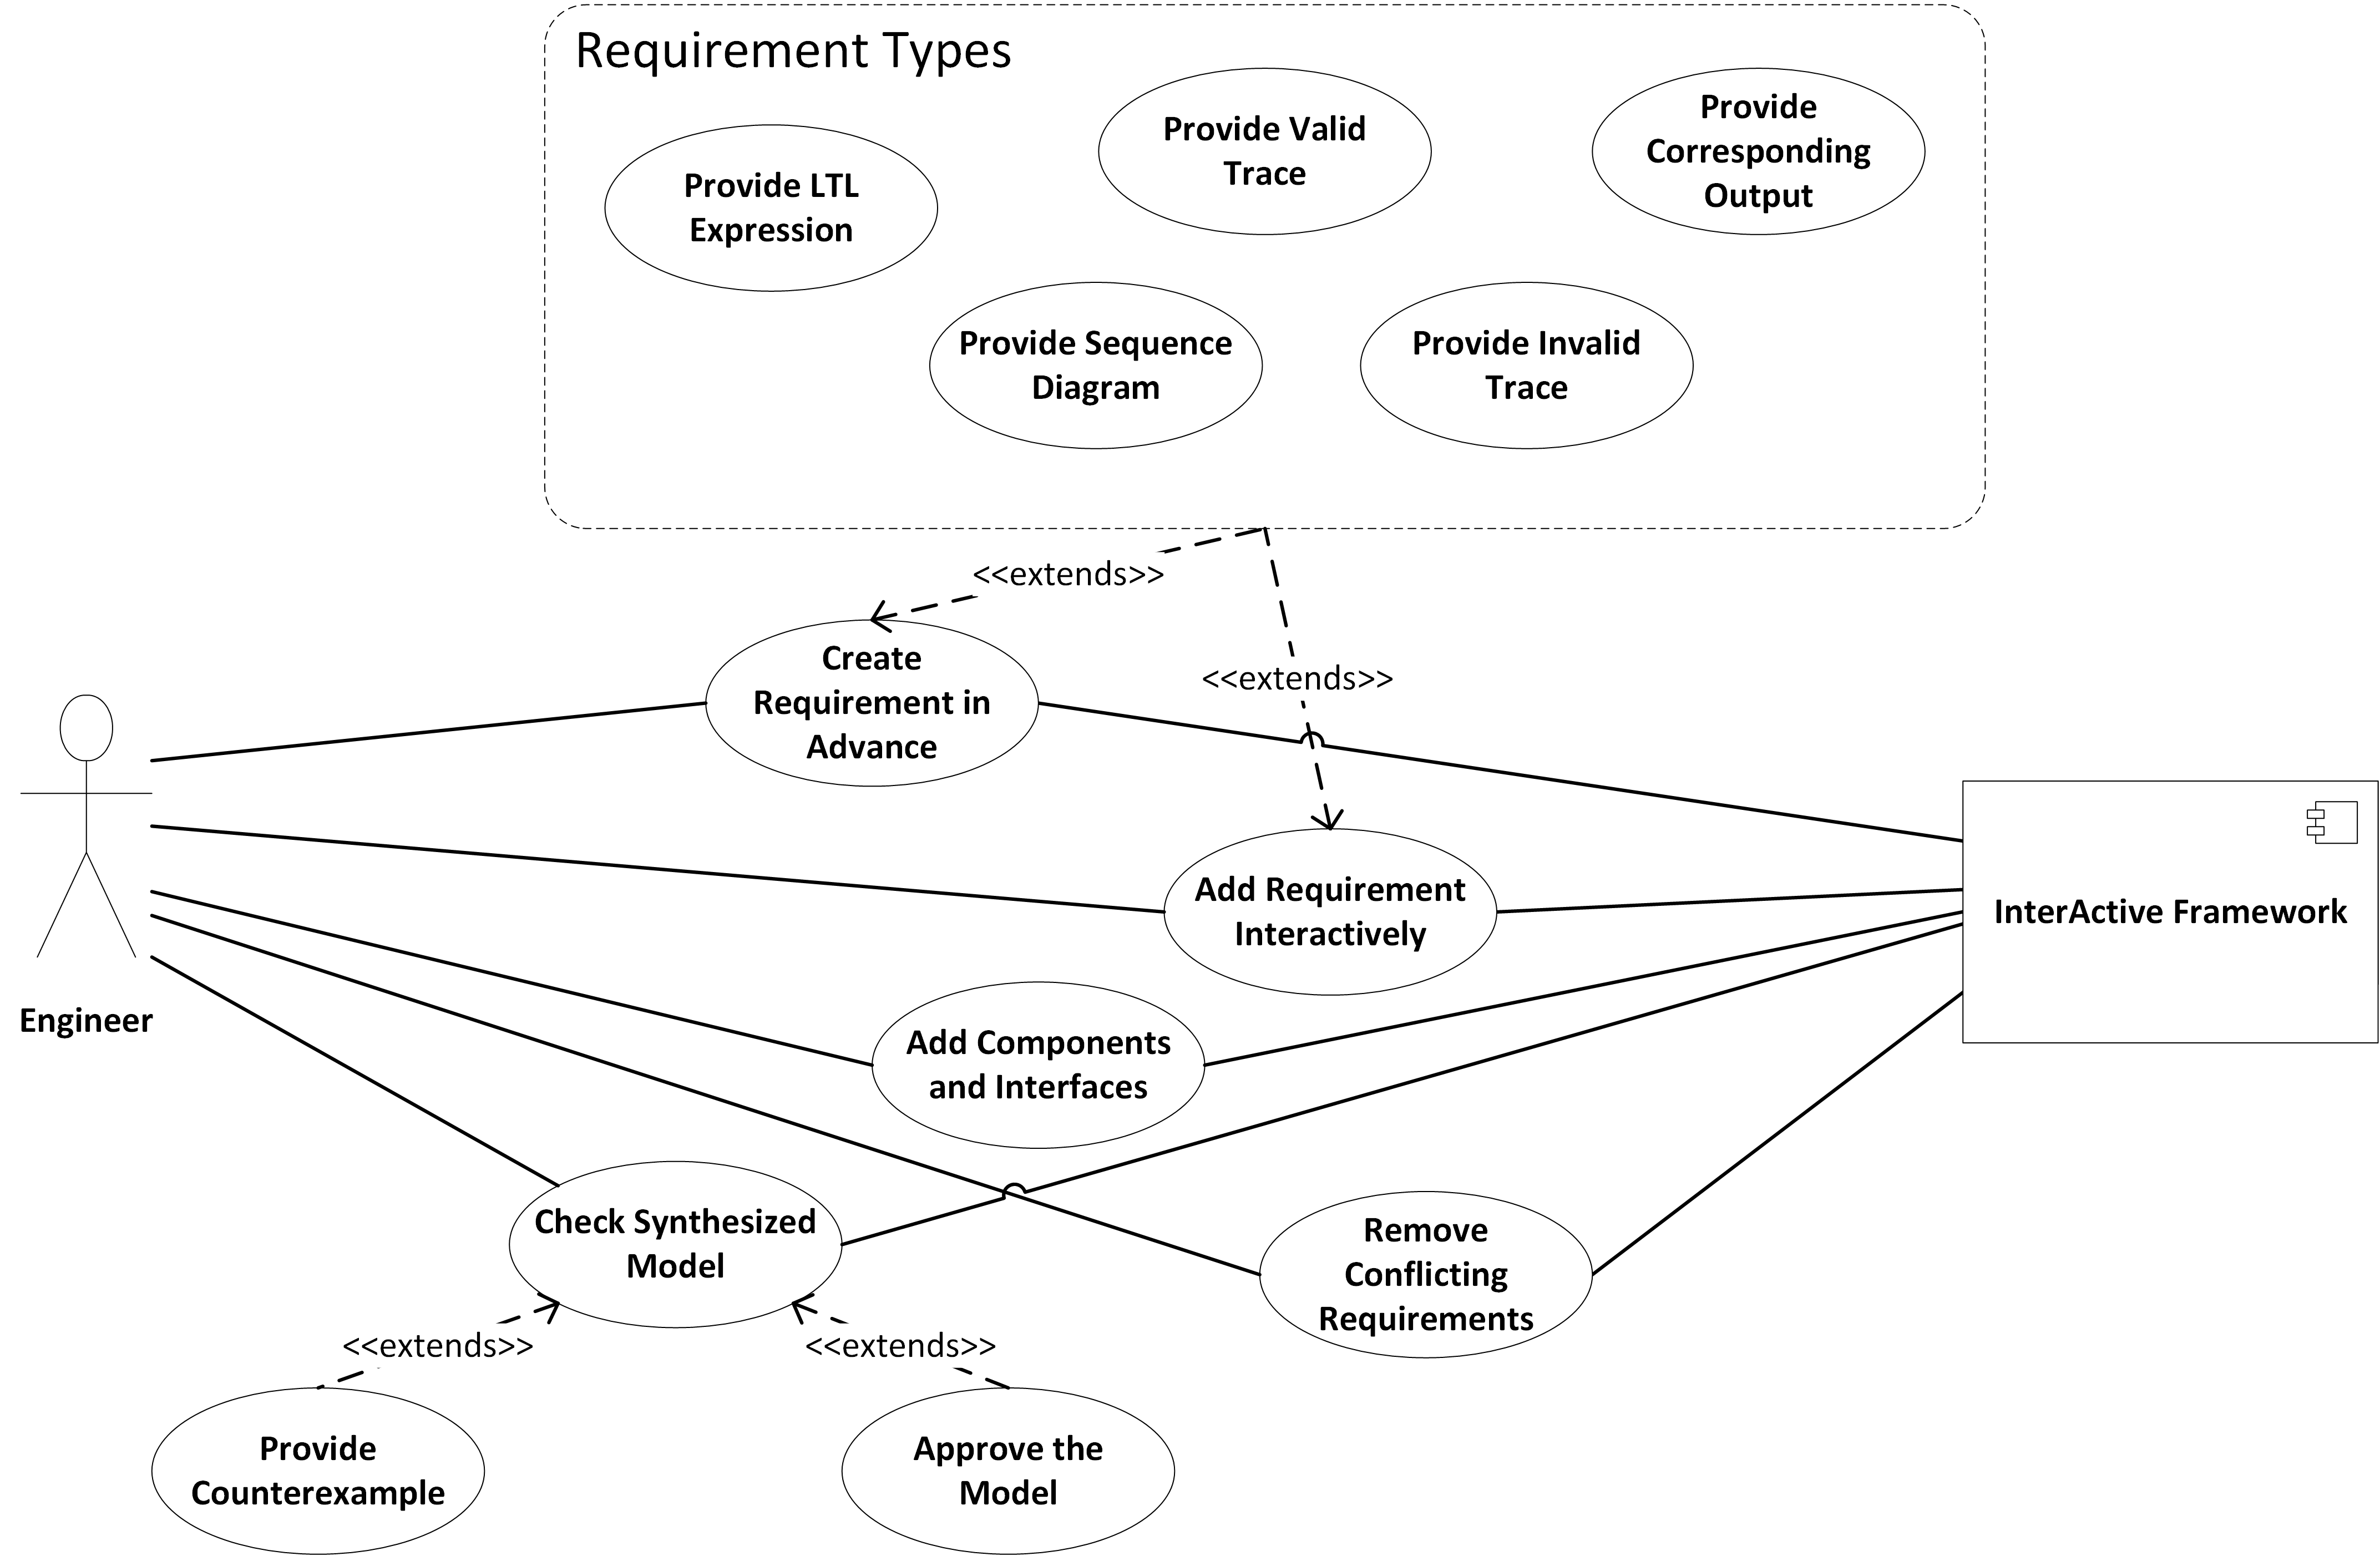
\includegraphics[width=100mm, keepaspectratio]{figures/methodology_interactiontypes.png}
	%}
	\caption{Interaction types between the engineer and the ILE}
	\label{fig_methodology_interactiontypes}
\end{figure}

Our methodology is heavily based on the interaction of the user with the ILE. The different types of interacitons are summarized on Figure \ref{fig_methodology_interactiontypes} and are elaborated on in Subsection \ref{subs_reqtypes}. These interactions take place in a predefined order -- the \textit{proposed workflow}, illustrated on Figure \ref{fig_methodology_workflow}, the individual steps of which are explained in detail in the following subsections. This workflow consists of two phases: first, an \textit{offline} one, and then an \textit{online} one, and ends with the serialization of the models. During the offline phase, the ILE offers little assistance, the designing engineer must determine the required details by other means. The interactive system design happens during the online phase. 

The input formalisms of individual steps in both the offline and the online phases have a predefined syntax with the corresponding, precisely defined semantics. Their common feature is the declarative way of describing the system components, which allows the engineer to focus solely on the expected behavior and acquire a minimal model exhibiting the specified functionality.

\begin{figure}[!ht] 
	\centering
	\fbox{
		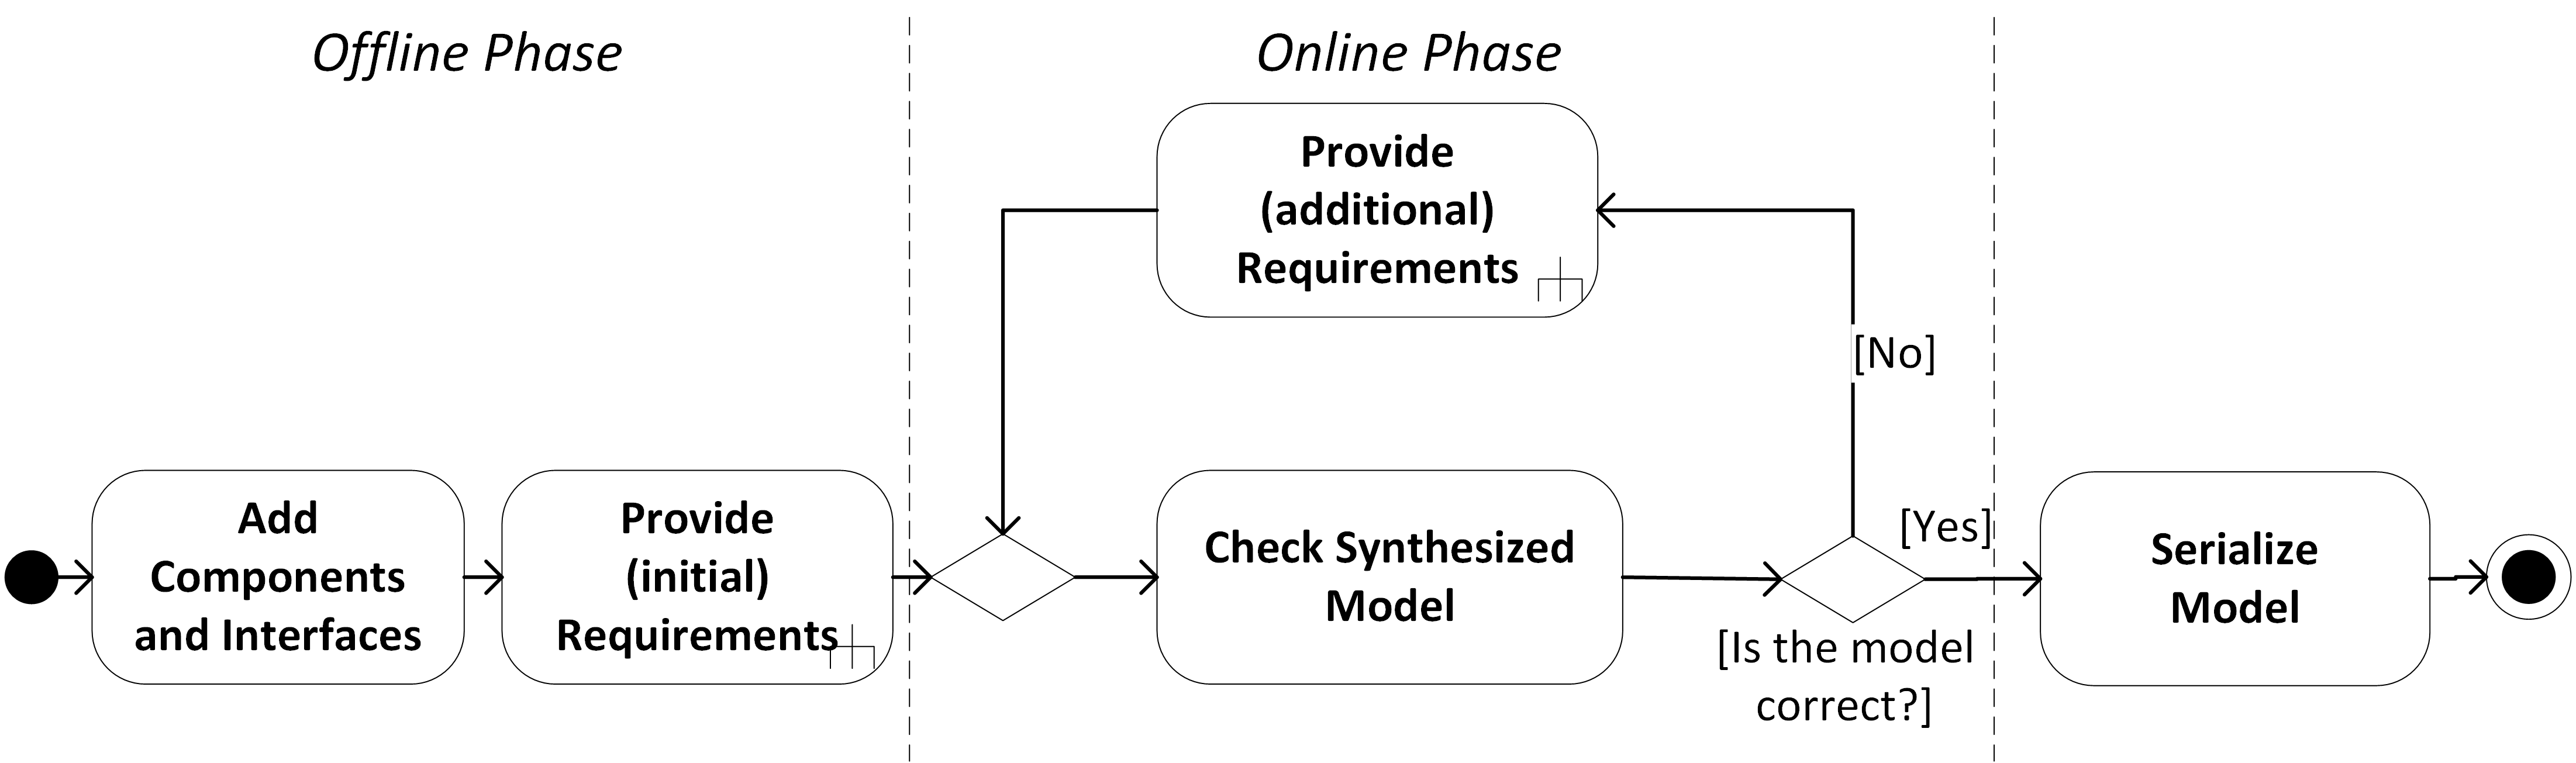
\includegraphics[width=150mm, keepaspectratio]{figures/methodology_workflow.png}
	}
	\caption{The Proposed Workflow}
	\label{fig_methodology_workflow}
\end{figure}

%---------------------------------------------------------------
\subsection{Component and Interface Definition} \label{subs_compdef}
%---------------------------------------------------------------
The first step of the workflow is the definition of the system components. This happens in the offline phase, as the determination of the system components, their exact boundaries and interfaces is part of the architecture, not the behavior. The engineer must provide the names of the system components, along with their interfaces -- in other words their input- and output alphabets -- before the workflow can proceed to the next step.

Users are encouraged to specify input and output characters qualified with port names in the format '{\fontfamily{qcr}\selectfont Port.character}', as this supplies the subsequent steps with essential information about the connections of the individual system components.

The components are handled as independent systems in every other aspect. This results - among others - in the arbitrary ordering of the online behavior-learning phases, and the behavioral faults being limited to their components of origin (although this does not limit the propagation of errors through messages resulting from incorrect behavior).
The syntax of component and interface declarations is quite simple, as illustrated in Listing \ref{lst_compdef}.

\bigskip
\begin{lstlisting} [language=tex,caption=Example of a component declaration along with its interfaces,label=lst_compdef]
	Please provide the system components (space-separated):
	>TrafficLight
	Please provide the input alphabet for component TrafficLight (space-separated):
	>TrafficControl.interrupt TrafficControl.toggle
	Please provide the output alphabet for component TrafficLight (space-separated):
	>TrafficDisplay.red TrafficDisplay.yellow TrafficDisplay.green TrafficDisplay.blinkingYellow
\end{lstlisting}

%---------------------------------------------------------------
\subsection{Requirement Types} \label{subs_reqtypes}
%---------------------------------------------------------------
During the workflow, the engineers can provide requirements in both phases. These requirements can vary greatly in their scope -- from being specific to individual runs to being generally valid for the whole component -- in addition to the differences in the formalism the user defines them through. 

In the offline phase, this means that the users add requirements they have formulated in advance. This is useful for more general requirements, with the scope of the whole component, easily formulated as program logic expressions, or long and complex traces.

In the online phase, adding requirements means answering the questions formulated by the algorithm about a yet unspecified behavior at a specific place in the trace currently being examined. This too can be answered through program logic - e.g. when the engineer realizes a general property during the model construction - but also through traces and through giving the corresponding output directly.

The currently supported requirement types can be seen on Figure \ref{fig_requirementtypes}.

\begin{figure}[!ht] 
	\centering
	%\fbox{
		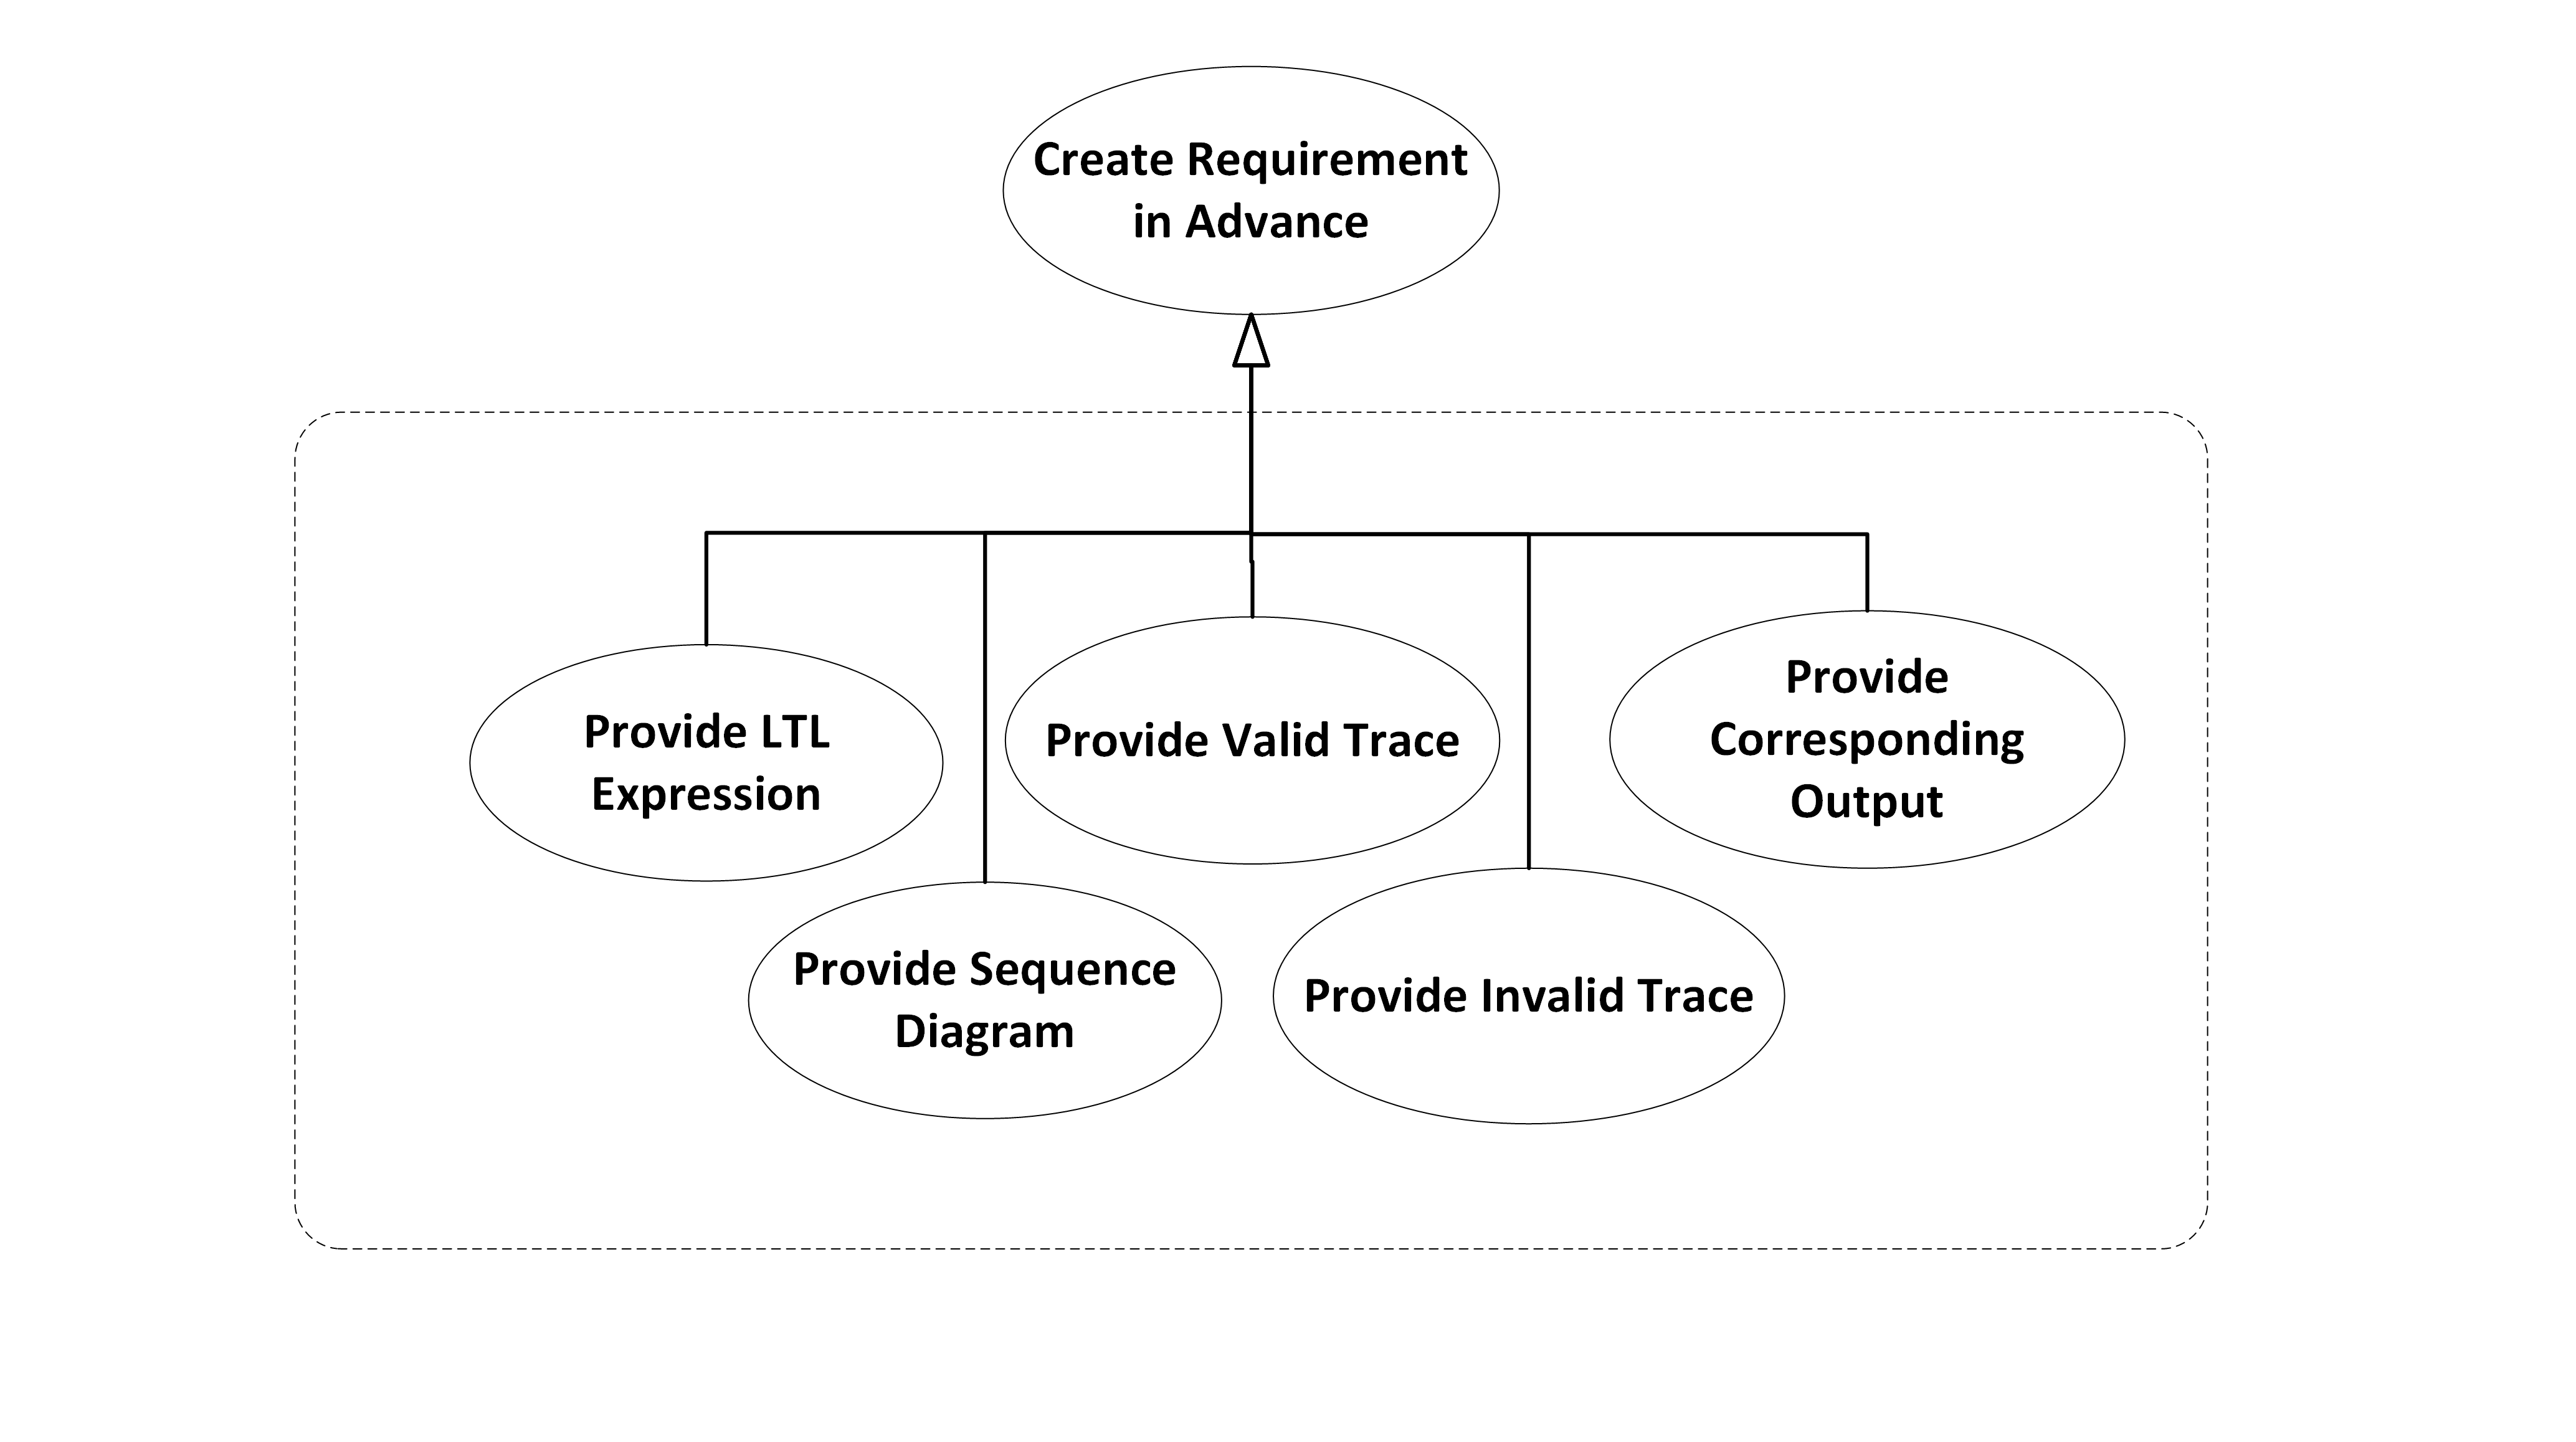
\includegraphics[width=130mm, keepaspectratio]{figures/methodology_requirementtypes.png}
	%}
	\caption{The supported requirement types}
	\label{fig_requirementtypes}
\end{figure}

\textbf{Corresponding Output}

This is the simplest way of specifying the behavior of the system, also containing the least amount of information among the different model types. To put simply, this means giving the output for a given input sequence, without any additional information. This supposedly answers the question of the ILE at \textit{one} given point, and that is the end of its scope.

Examples of corresponding output specification can be seen in Listing \ref{lst_iopair}. The alphabets of the component are the ones defined in in Listing \ref{lst_compdef}.

\bigskip
\begin{lstlisting} [language=tex,caption=Examples of corresponding output specification,label=lst_iopair]
	Offline: 
	// choosing the type of the requirement omitted
	>TrafficControl.toggle TrafficControl.toggle TrafficControl.toggle/TrafficDisplay.yellow
	
	Online: 
	Unknown output for input sequence [TrafficControl.toggle TrafficControl.toggle TrafficControl.toggle]:
	// choosing the type of the requirement omitted
	>TrafficDisplay.yellow
\end{lstlisting}

\textbf{Valid Trace}

Valid traces contain information about multiple related input sequences, as they provide the corresponding output for any prefix of the contained input sequence. This can be useful, as the engineers often take the whole output sequence into consideration when determining the output for some inputs. Thus, the ILE can obtain \textit{multiple} answers concerning the behaviors in question by automated means, saving on the number of required interactions with the user.

Examples can be seen in Listing \ref{lst_validtrace}, assuming the previously used alphabets.

\bigskip
\begin{lstlisting} [language=tex,caption=Examples of a valid trace specifications,label=lst_validtrace]
	Offline:
	// choosing the type of the requirement omitted
	>TrafficControl.toggle/TrafficDisplay.red TrafficControl.toggle/TrafficDisplay.green TrafficControl.toggle/TrafficDisplay.yellow
	
	Online: 
	Unknown output for input sequence [TrafficControl.interrupt]:
	// choosing the type of the requirement omitted
	>TrafficControl.interrupt/TrafficDisplay.blinkingYellow TrafficControl.interrupt/TrafficDisplay.red TrafficControl.interrupt/TrafficDisplay.blinkingYellow
\end{lstlisting}

\textbf{Invalid Trace}

Invalid traces are similar to valid traces, with the difference that the contained behavior must not appear in the resulting model -- thus defining traces to exclude. They are most useful for small output alphabets, or when the range of possible behaviors is otherwise contained - e.g. through program logic expressions or several other excluded traces.

They can also be used to check the hidden implications of other requirements: trace-based models are easy to construct and the ILE will signal any conflicts with other, more complex requirements of which the engineer may not see the hidden implications.

Examples for invalid traces can be seen in Listing \ref{lst_invalidtrace}. Notice, that invalid traces have the same syntax as valid traces, the difference is in their semantics.

\bigskip
\begin{lstlisting} [language=tex,caption=Example of a trace to exclude,label=lst_invalidtrace]
	Offline:
	// choosing the type of the requirement omitted
	>TrafficControl.interrupt/TrafficDisplay.green TrafficControl.interrupt/TrafficDisplay.yellow
	
	Online:
	Unknown output for input sequence [TrafficControl.interrupt]:
	// choosing the type of the requirement omitted
	>TrafficControl.interrupt/TrafficDisplay.green TrafficControl.interrupt/TrafficDisplay.yellow TrafficControl.interrupt/TrafficDisplay.red
\end{lstlisting}

\textbf{Sequence Diagram}

UML-like sequence diagrams are trace-based models that can contain multiple traces, due to them having various combined fragments for branching the behavior - like \textit{alt} and \textit{opt} - and for referencing behaviors specified elsewhere - like \textit{ref}.

Sequence diagrams can also be used to model arbitrarily long, possibly looping behavior, thereby containing plenty of information, which results in possibly answering \textit{numerous} questions formulated by the ILE.

We introduce our own sequence diagram formalism specifically designed to model system components. An example for their syntax can be seen on Figure \ref{fig_sequencediagram}. The '\textit{systemComponent}' is the component the behavior of which is being modeled, the '\textit{inputComponent}' and '\textit{outputComponent}' are symbolizing the sources and targets of the inputs and outputs. The textboxes marked with stars are the port qualifications.

\begin{figure}[!ht] 
	\centering
	%\fbox{
	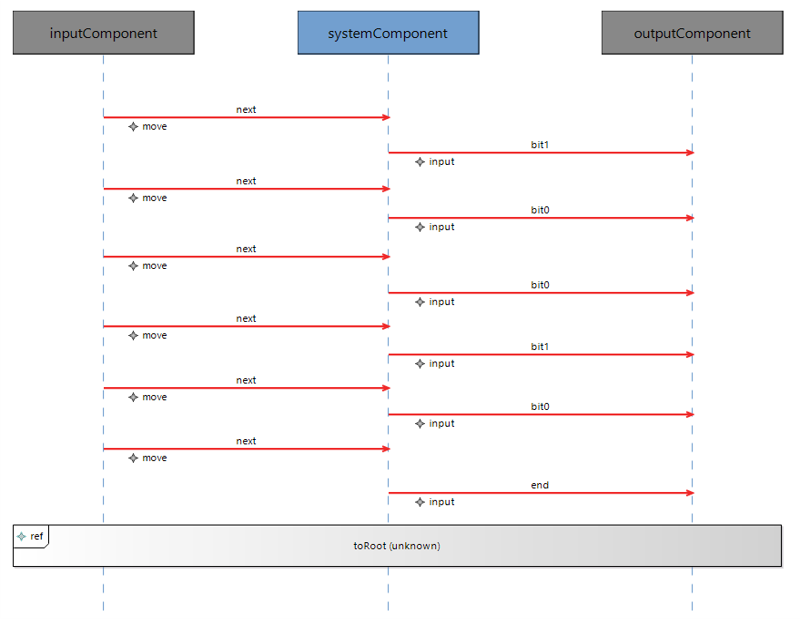
\includegraphics[width=130mm, keepaspectratio]{figures/sequencediagram.png}
	%}
	\caption{Example for the syntax of the sequence diagrams}
	\label{fig_sequencediagram}
\end{figure}


It is important to note, that the specification and integration of sequence diagrams into this framework is not yet complete. 

\textbf{LTL Expression}

LTL expressions are able to contain infinitely many traces through program logic-based requirement specification: they can be used to formulate propositional logic expressions with temporal connectives over \textit{paths} of a \textit{base model}, as described in Subsection \ref{subs_backgrltl}. 

They can be used to formulate requirements that must hold for the whole component, during the whole execution. Thus -- depending on their interpretation -- they contain lots of information, which may result in answering \textit{numerous} questions posed by the ILE.

For our application, we introduce our own LTL expression language with its own syntax and semantics - although attempting to keep it similar to other generally known variants, especially that of SPOT \cite{Spot}. The full syntax of the LTL expressions -- also determining the operator precedence -- can be seen in Listing \ref{lst_ltlfullsyntax} in the Appendix.

The base model of the LTL expressions is the LTS interpretation of the component under learning. This means, that the set of atomic propositions that can be used in these expressions are the possible labels of the transitions, which are the elements of the input and the output alphabets of the component. The model synthesis takes place assuming \textit{event semantics} -- exactly one input and one output event happening at any given step during the execution of the system. We introduced these semantics to the LTL expressions: the conjunction of exactly one input and one output character must hold at any given point for it to be considered correct -- and every other character must be negated at the same point. This also entails, that given another character not explicitly negated at that point, it is automatically negated, and in case that no proposition is declared explicitly, either one of the non-explicitly negated characters hold. 

The semantics of the supported temporal connectives, and other aspects of the LTL semantics in general, are similar to those described in Subsection \ref{subs_backgrltl}.

Examples for LTL expressions can be seen in Listing \ref{lst_ltlex}.

\bigskip
\begin{lstlisting} [language=tex,caption=Examples of LTL expressions,label=lst_ltlex]
	Offline:
	// choosing the type of the requirement omitted
	>F(TrafficControl.interrupt -> X(G(TrafficControl.toggle) -> G(TrafficDisplay.blinkingYellow)))

	Online: 
	Unknown output for input sequence [TrafficControl.interrupt TrafficControl.toggle]:
	// choosing the type of the requirement omitted
	>F(TrafficControl.interrupt -> X(G(TrafficControl.toggle) -> G(TrafficDisplay.blinkingYellow)))
	
	Equivalent as a result of the event semantics (omitting port qualifications for simplicity):
	>F(interrupt&!toggle -> X(G(toggle&!interrupt) -> G(blinkingYellow&!red&!green&!yellow)))
\end{lstlisting}

It is important to note, that the specification of our LTL variant is not yet finished.

%---------------------------------------------------------------
\subsection{Conflicting Requirements} \label{subs_conf}
%---------------------------------------------------------------
The requirements provided by the designing engineer to the ILE may easily be conflicting, especially in case of LTL expressions and invalid traces that describe arbitrarily long sets of behaviors. This is expected, as during system design, when the engineer refines the models and reaches lower levels of abstraction, certain scenarios may conflict with some oversimplified conditions. At that point, those too must be refined, thus replaced. This is why it is essential for the system to provide some kind of conflict handling within the practical boundaries of the available resources. 

This problem is a difficult and resource intensive task for algorithmic reasons elaborated later. Consequently, the ILE only guarantees to handle the conflict, when it also interferes with the model synthesis, in which case, the user is asked to remove one of the conflicting models, before the analysis of the behavior can proceed -- as shown on Figure \ref{fig_providerequirementsworkflow}.

\begin{figure}[H] 
	\centering
	%\fbox{
		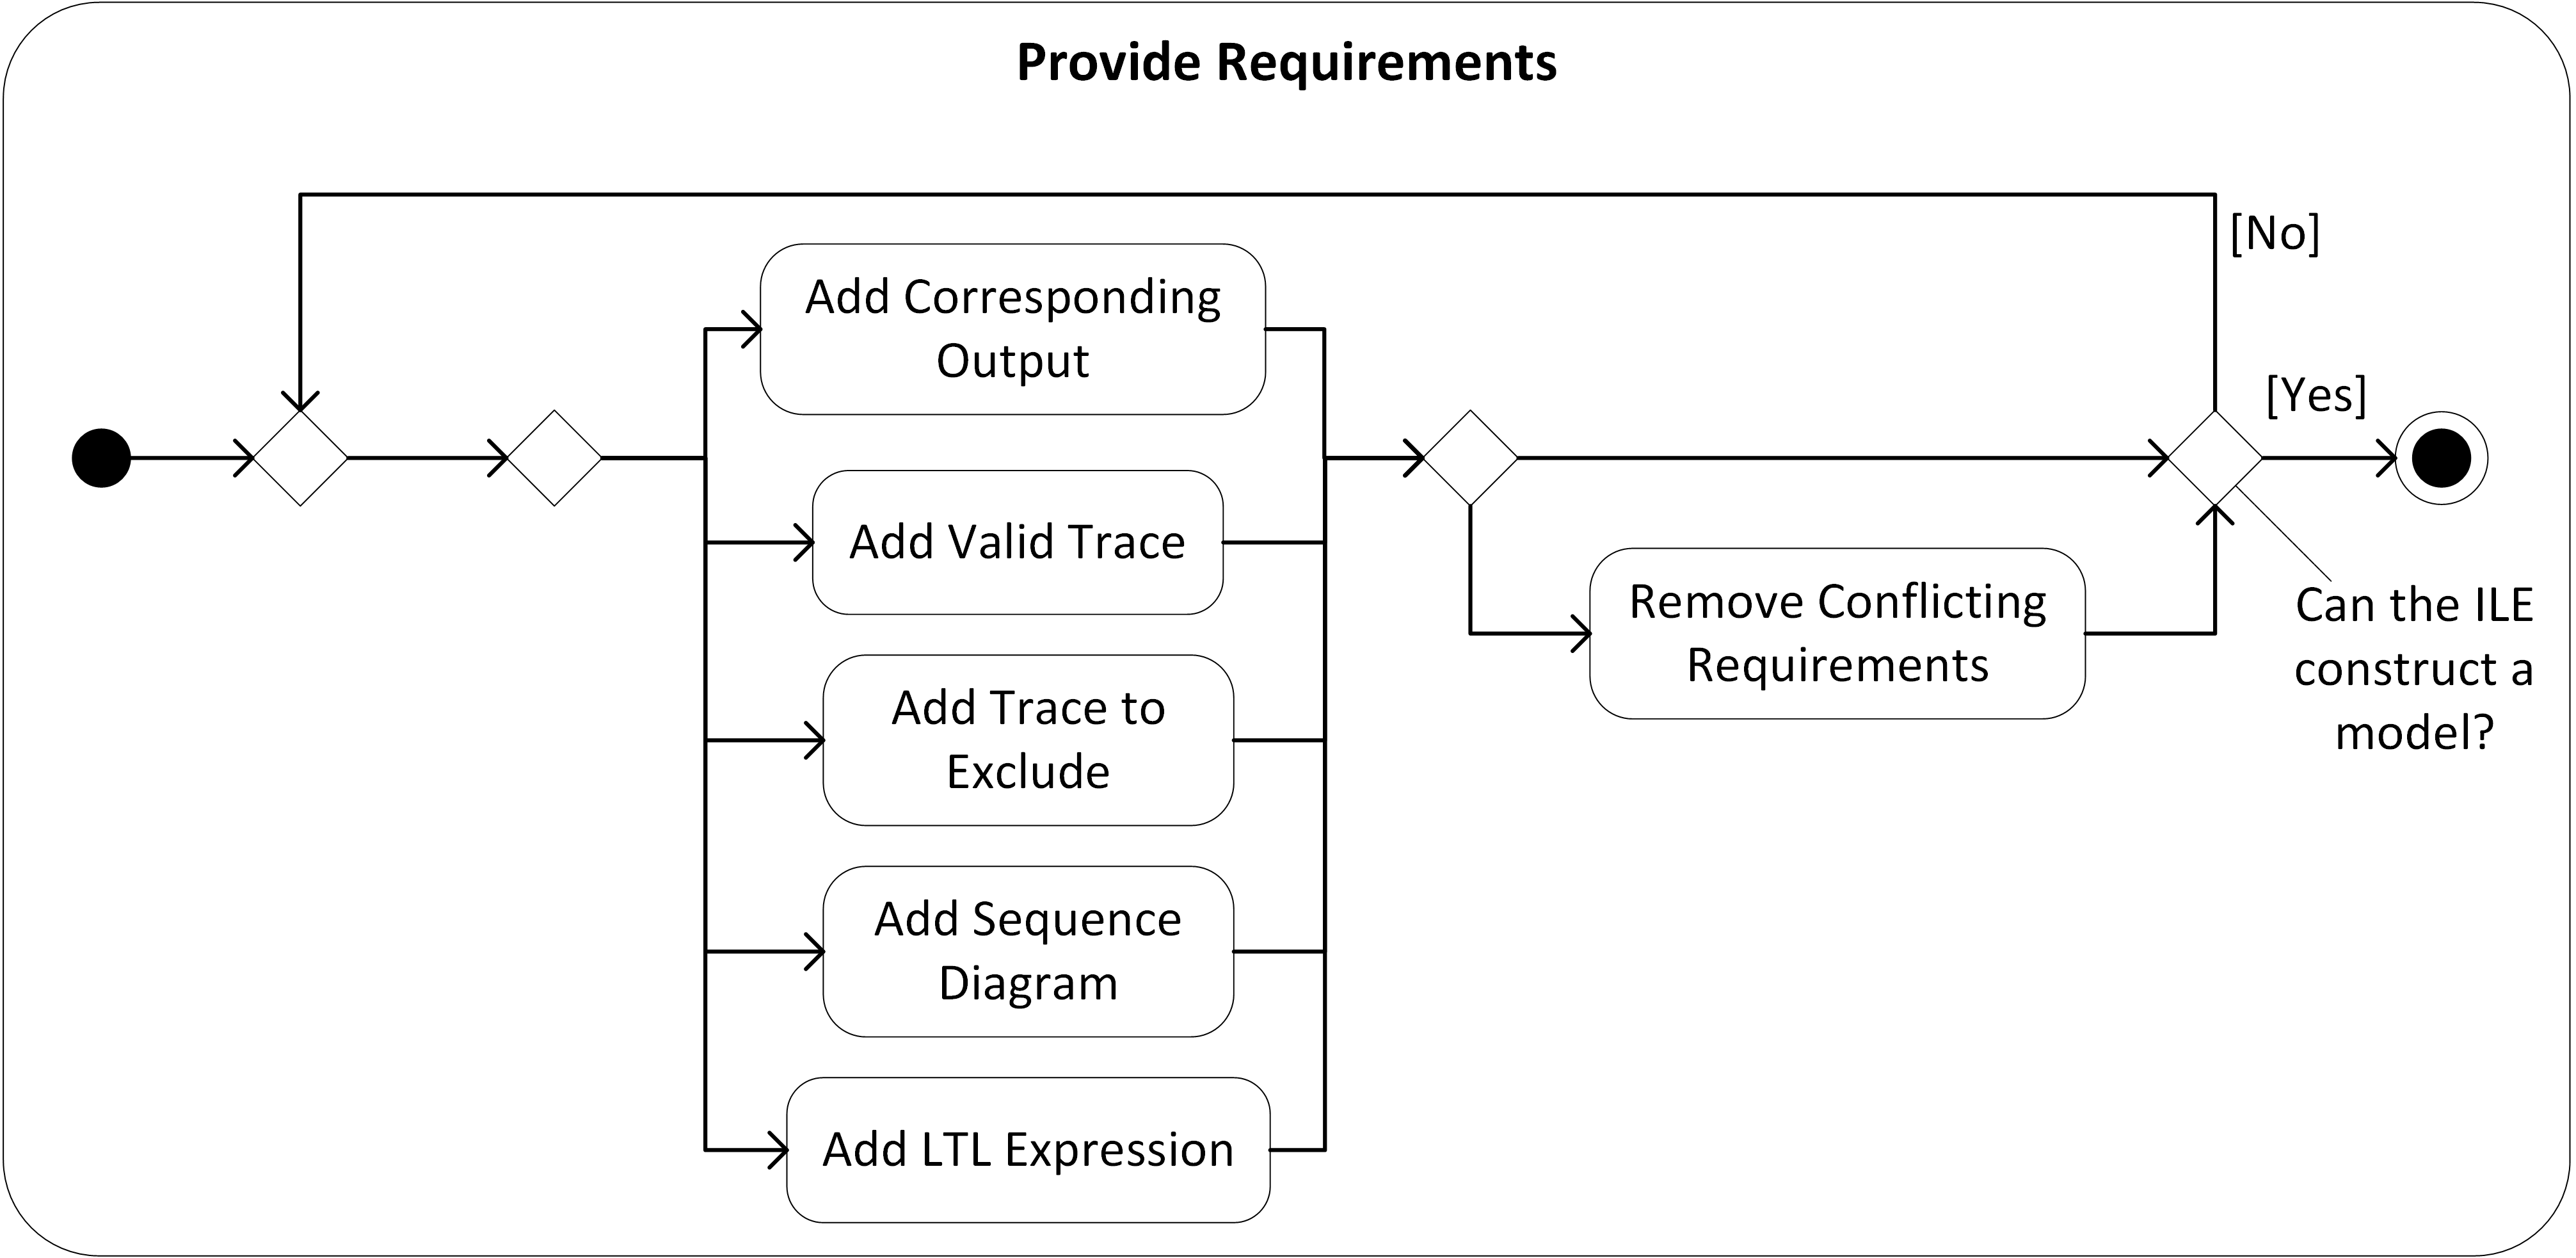
\includegraphics[width=130mm, keepaspectratio]{figures/methodology_providerequirementsworkflow.png}
	%}
	\caption{The process of adding a requirement}
	\label{fig_providerequirementsworkflow}
\end{figure}


As conflicts only become apparent during the online phase of the workflow, that is where the conflicts have to be handled. However, conflicts that were introduced earlier are also discovered and resolved in that phase. An example of a requirement conflict handling can be seen in Listing \ref{lst_conflicthandling}.

\bigskip
\begin{minipage}{\linewidth}
\begin{lstlisting} [language=tex,caption=Example of a requirement conflict handling,label=lst_conflicthandling]
	Models 1) IO Pair Model: [TraffiControl.interrupt]/TrafficDisplay.red and 0) Invalid Trace Model: TrafficControl.interrupt/TrafficDisplay.red are conflicting.
	Please choose which model to remove: 
	>1			//this removes the I/O pair model
\end{lstlisting}
\end{minipage}

%---------------------------------------------------------------
\subsection{Checking the Correctness of the Synthesized Model} \label{subs_eq}
%---------------------------------------------------------------
During the online phase, whenever the ILE assumes that it has gathered enough information to construct a model for the given component, the engineer if offered with a model representing the current state of the model synthesis -- the equivalent of an equivalence query in automata learning algorithms. The user can either approve this model -- in which case the automata learning and therefore the designing of the behaviour is complete -- or provide a counterexample where the model does not meet the -- not yet specified -- requirements.

The proposed equivalence model is a deterministic automaton, which, based on the information provided by the user, can be incomplete in multiple ways. The behavior of the desired model can differ from that of the learned system because of lacking information, in which case the user (acting as the equivalence oracle of the learning) needs to provide the separating behavior. Another reason for incompleteness can be newly discovered states, whose behavior is unknown based on their input signatures. This case prompts the user to evaluate the validity of state separation and to provide the lacking information. If, for some reason the hypothesized behavior is contradicting that of the desired system (by the users oversight in providing requirements), the actual, conflicting requirement can be provided to guide the learning algorithm through the process described in Subsection \ref{subs_conf}.

If the model is accepted, the design phase is complete and the model is serialized. If a counterexample is provided, the online phase resumes and the system design continues until the next possible model is reached.

Examples of models offered in equivalence queries can be seen on Figure \ref{fig_methodology_eqex}.

\begin{figure}[H] 
	\centering
	\fbox{
		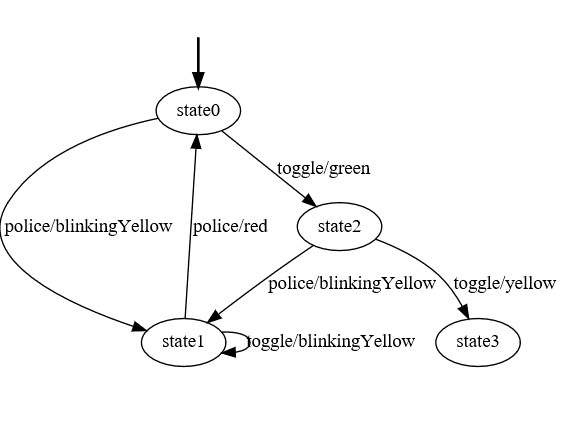
\includegraphics[height=50mm, keepaspectratio]{figures/methodology_eqex1.png}
	}
	\fbox{
		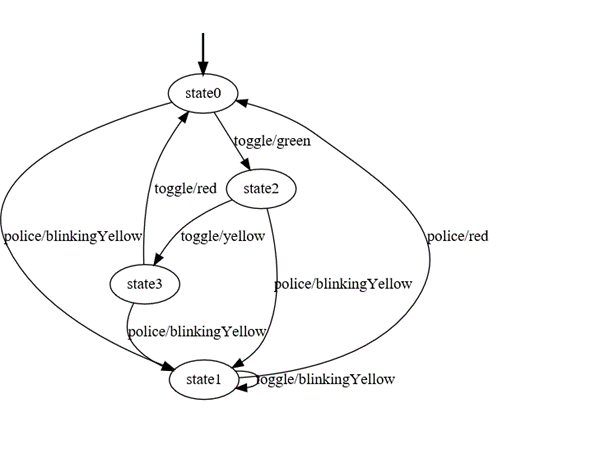
\includegraphics[height=50mm, keepaspectratio]{figures/methodology_eqex2.png}
	}
	\caption{Equivalence query for an incomplete model (\textit{left}) and the final model (\textit{right})}
	\label{fig_methodology_eqex}
\end{figure}

%---------------------------------------------------------------
\subsection{The Resulting System Model} \label{subs_resultingmodel}
%---------------------------------------------------------------
When each of the component models declared during the first step of the workflow are completed, the resulting system model can be serialized and handed over to the engineer for further extensions or usage, e.g. for code generation. The serialization can happen in various formalisms.

A possible formalism is the Gamma statechart, introduced in \cite{DBLP:conf/icse/MolnarGVMV18}. Gamma statecharts are high-level state-based models, to which every functionality offered by the Gamma Statechart Composition Framework can be applied. Our framework offers full-scale Gamma serialization: when choosing this formalism, a whole project will be created, along with interface definitions, component definitions - for each of the previously declared components, with the synthesized behavior - and a composite system definition, connecting the components based on the names of their ports.

Another possibility is the serialization to the Mealy machine formalism of the framework - as presented when checking the correctness of the model. This results in a lower-level set of independent models, with a completely different set of applications.

\clearpage
%----------------------------------------------------------------------------
\section{Overview of the Architecture} \label{sec_architecture}
%----------------------------------------------------------------------------

The architecture of the ILE consists of two main components: the learning algorithm - which is responsible for the model synthesis procedure, thus the course of the learning - and the interactive oracle - investigating the membership of the given input sequences in the languages of the models given by the user on one side and interacting with the user on the other. A functional overview of this architecture is depicted on Figure \ref{fig_architcture_informaloverview}. The following subsections elaborate on the connections and details of these components.

\begin{figure}[!ht] 
	\centering
	\fbox{
		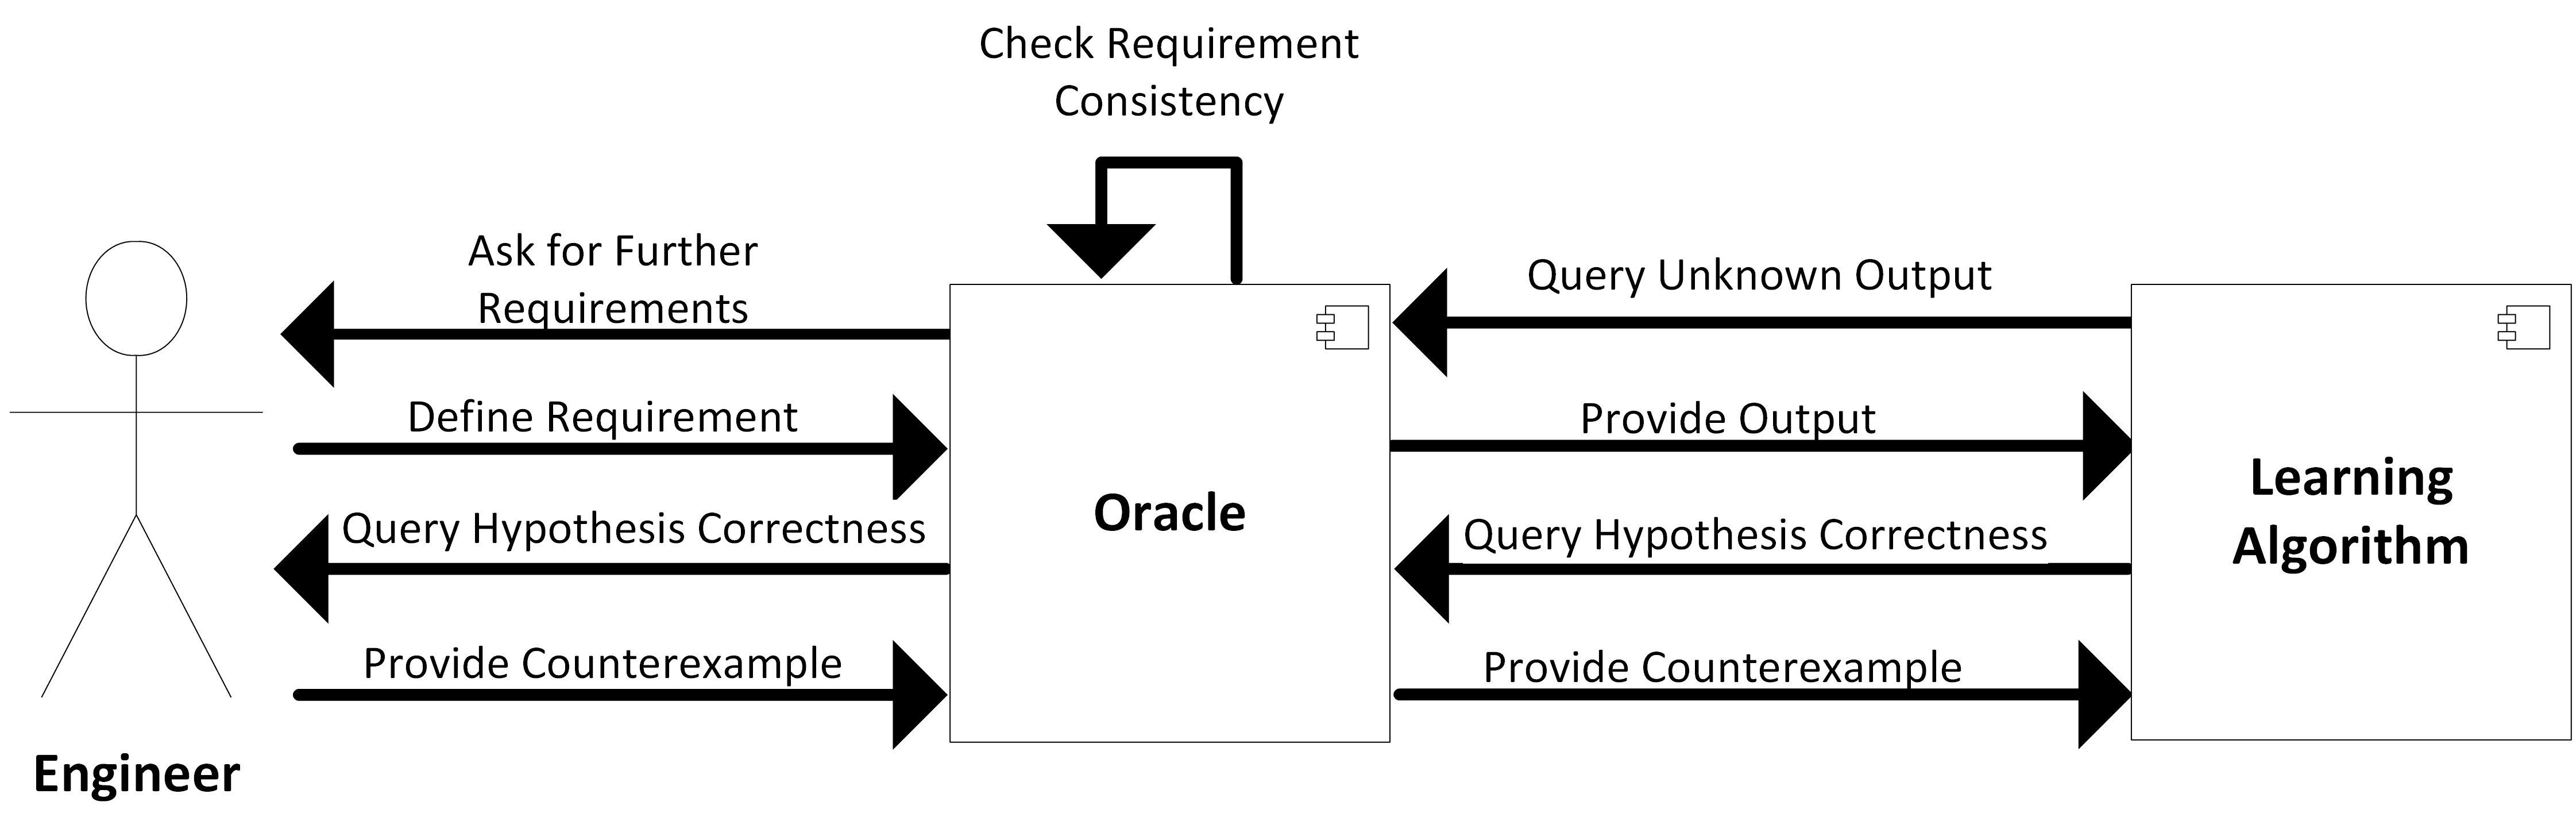
\includegraphics[width=140mm, keepaspectratio]{figures/architecture_informaloverview.png}
	}
	\caption{High-level architecture of the components of the ILE} 
	\label{fig_architcture_informaloverview}
\end{figure}

 In the case of the learning algorithm, active automata learning algorithms were chosen as a design direction. Active automata learning enables complete separation of the learner algorithm and the system under learning through a teacher component -- enabling the system under learning to be made from multiple, separate requirement-models provided by the user. Since active automata learning works through queries, the query can go through arbitrary layers of logic -- allowing the proposed oracle-based interactive learning.
 
 \smallskip

 As discussed in Chapter \ref{background}, active automata learning algorithms work through a teacher and a learner component. While traditionally, the queries asked through the teacher are automated - by known or derived information and equivalence algorithms - in order to achieve an interactive algorithm, we created a new approach. Figure \ref{fig_architcture_informaloverview} shows the Learning Algorithm delegating its queries through the oracle, which delegates the questions to the user. The abstract approach presented in Figure \ref{fig_architcture_informaloverview} does enable interactive learning, but implementing it using traditional approaches (by delegating every single query to the user) proves to be infeasible in practical use cases because of the overwhelming amount of queries needed to learn a model. In order to overcome this boundary, we made optimizations to the ILE to automate a subset of queries, and we designed a new, \textit{adaptive} active automata learning approach to heuristically control the design space.

%---------------------------------------------------------------
\subsection{The Cost of Interaction} \label{subs_commandhandling}
%---------------------------------------------------------------

As discussed in the previous subsection, one of the most important cost metrics of the presented interactive learning architecture is the number of questions that reach the user. In order to minimize this, we propose a heuristic by which a decision can be made regarding which queries provide valuable information -- based on the currently defined requirements. Since active automata learning algorithms aren't equipped for such \textit{adaptive learning}, we created a new approach. 

Active learning algorithms generally assume that the information they require is readily available, and thus follow a "greedy" approach of querying. While this is appropriate for fully automated solutions, greedily exploring the design space can result in several magnitudes larger amount of previously unexplored queries, which do not necessarily provide new information, resulting in longer learning rounds (with more membership queries) exploring a larger amount of the behavior, and conversely less equivalence queries. To allow the designing engineer to validate the hypothesized model more frequently, and control of which unexplored behavior should be explored, a less greedy approach is required.

To solve the above issue, we introduce the concept of adaptive active automata learning, which uses types of behaviors - as illustrated in Figure \ref{fig_architcture_commandhandling} - as a heuristic to adaptively decide if and where a greedy approach should be taken. Already explored behaviors (e.g. previously queried, cached) as well as behaviors contained in the defined requirements can be answered in an automated way, allowing greediness. On the other hand, not specified behaviors should be explored in a more reserved manner, controlled by the user - not the automata learning algorithm. Based on the requirements outlined above, we defined three commands to control the adaption of such an algorithm.

\begin{itemize}
	\item $OPTIMISTIC$ (greedy) heuristic is used if the algorithm should follow a greedy approach in the next steps.
	\item $PESSIMISTIC$ (reserved) heuristic is used if the algorithm should not query the investigated behavior further.
	\item $RESET$ is used to re-start the learning if necessary.
\end{itemize}

\begin{figure}[!ht] 
	\centering
	\fbox{
		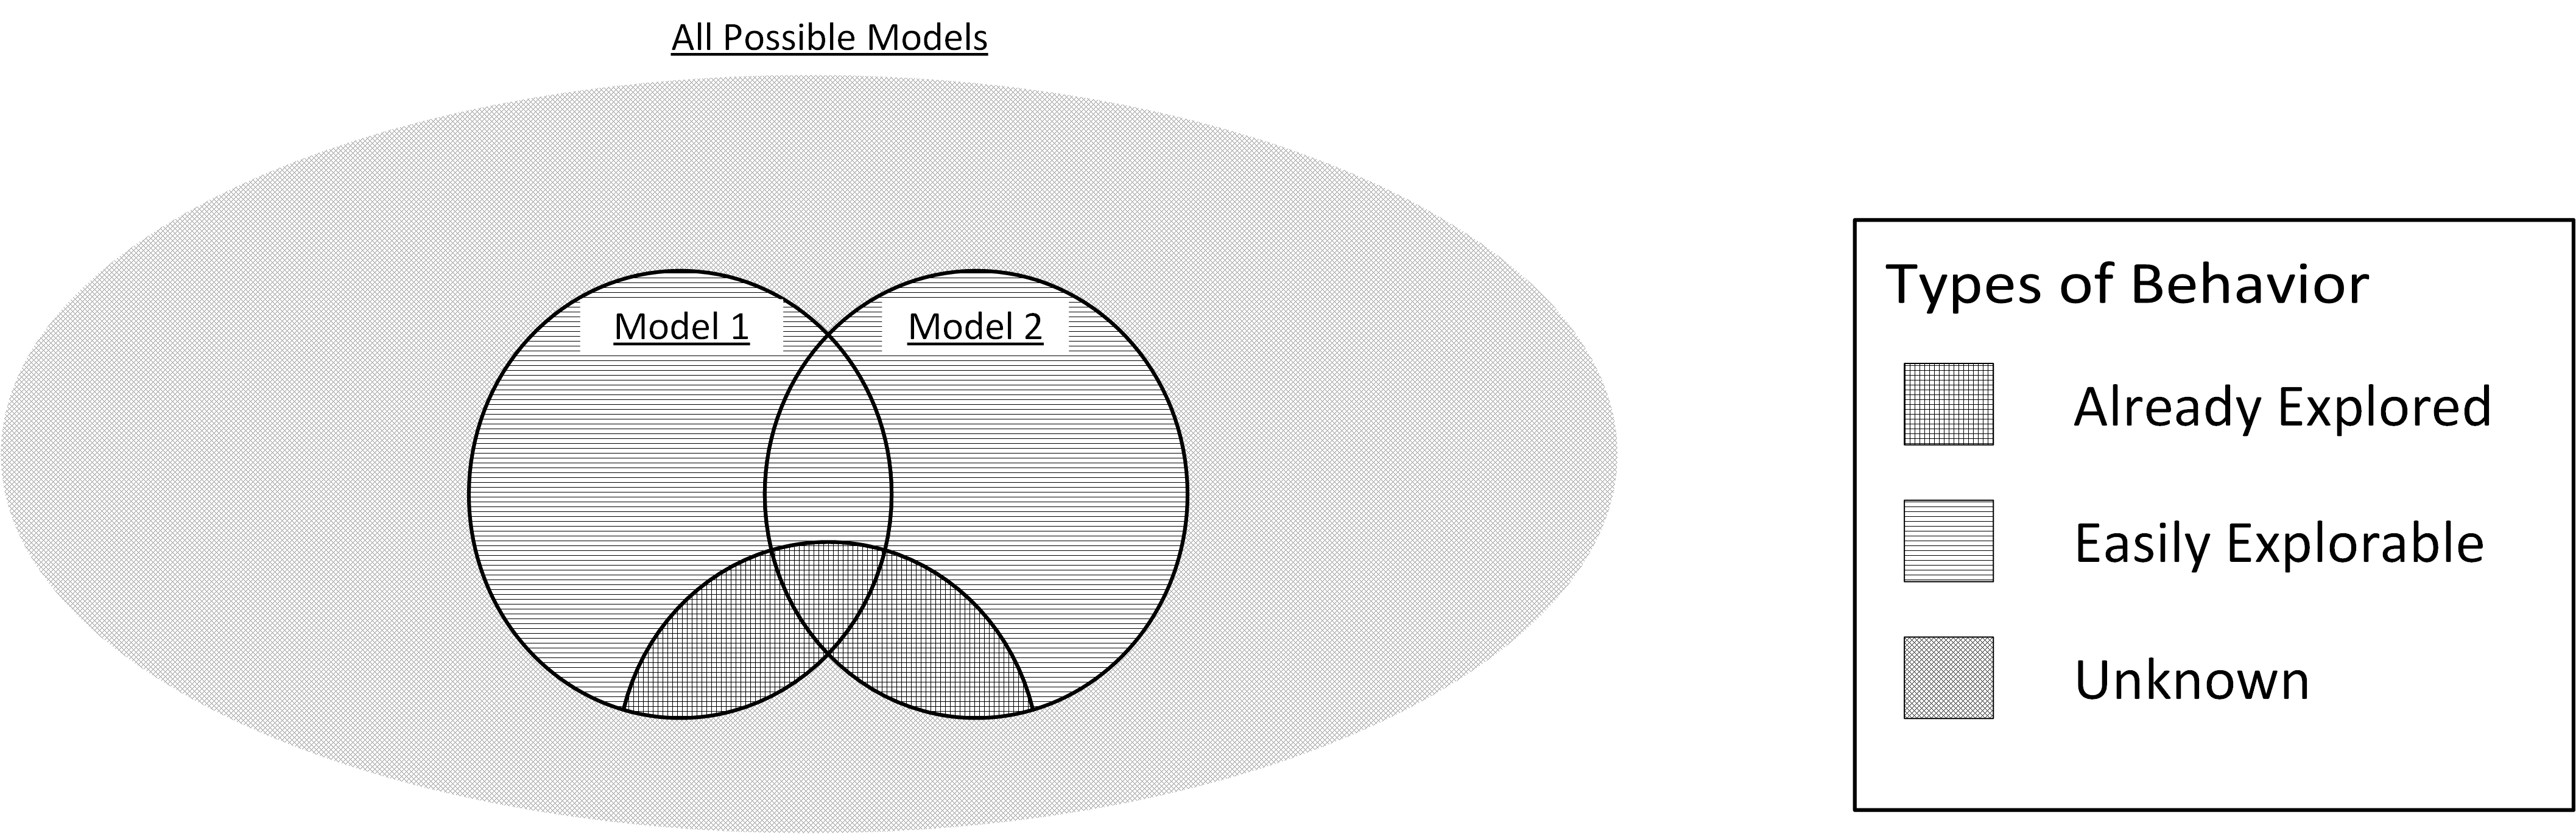
\includegraphics[width=150mm, keepaspectratio]{figures/architecture_commandhandling.png}
	}
	\caption{Types of behaviors during the learning process with two defined requirements} 
	\label{fig_architcture_commandhandling}
\end{figure} 



%---------------------------------------------------------------
\subsection{The Oracle} \label{subs_oracle}
%---------------------------------------------------------------

The architecture of the oracle component can be seen on Figure \ref{fig_architcture_oracle}.

\begin{figure}[!ht] 
	\centering
	%\fbox{
		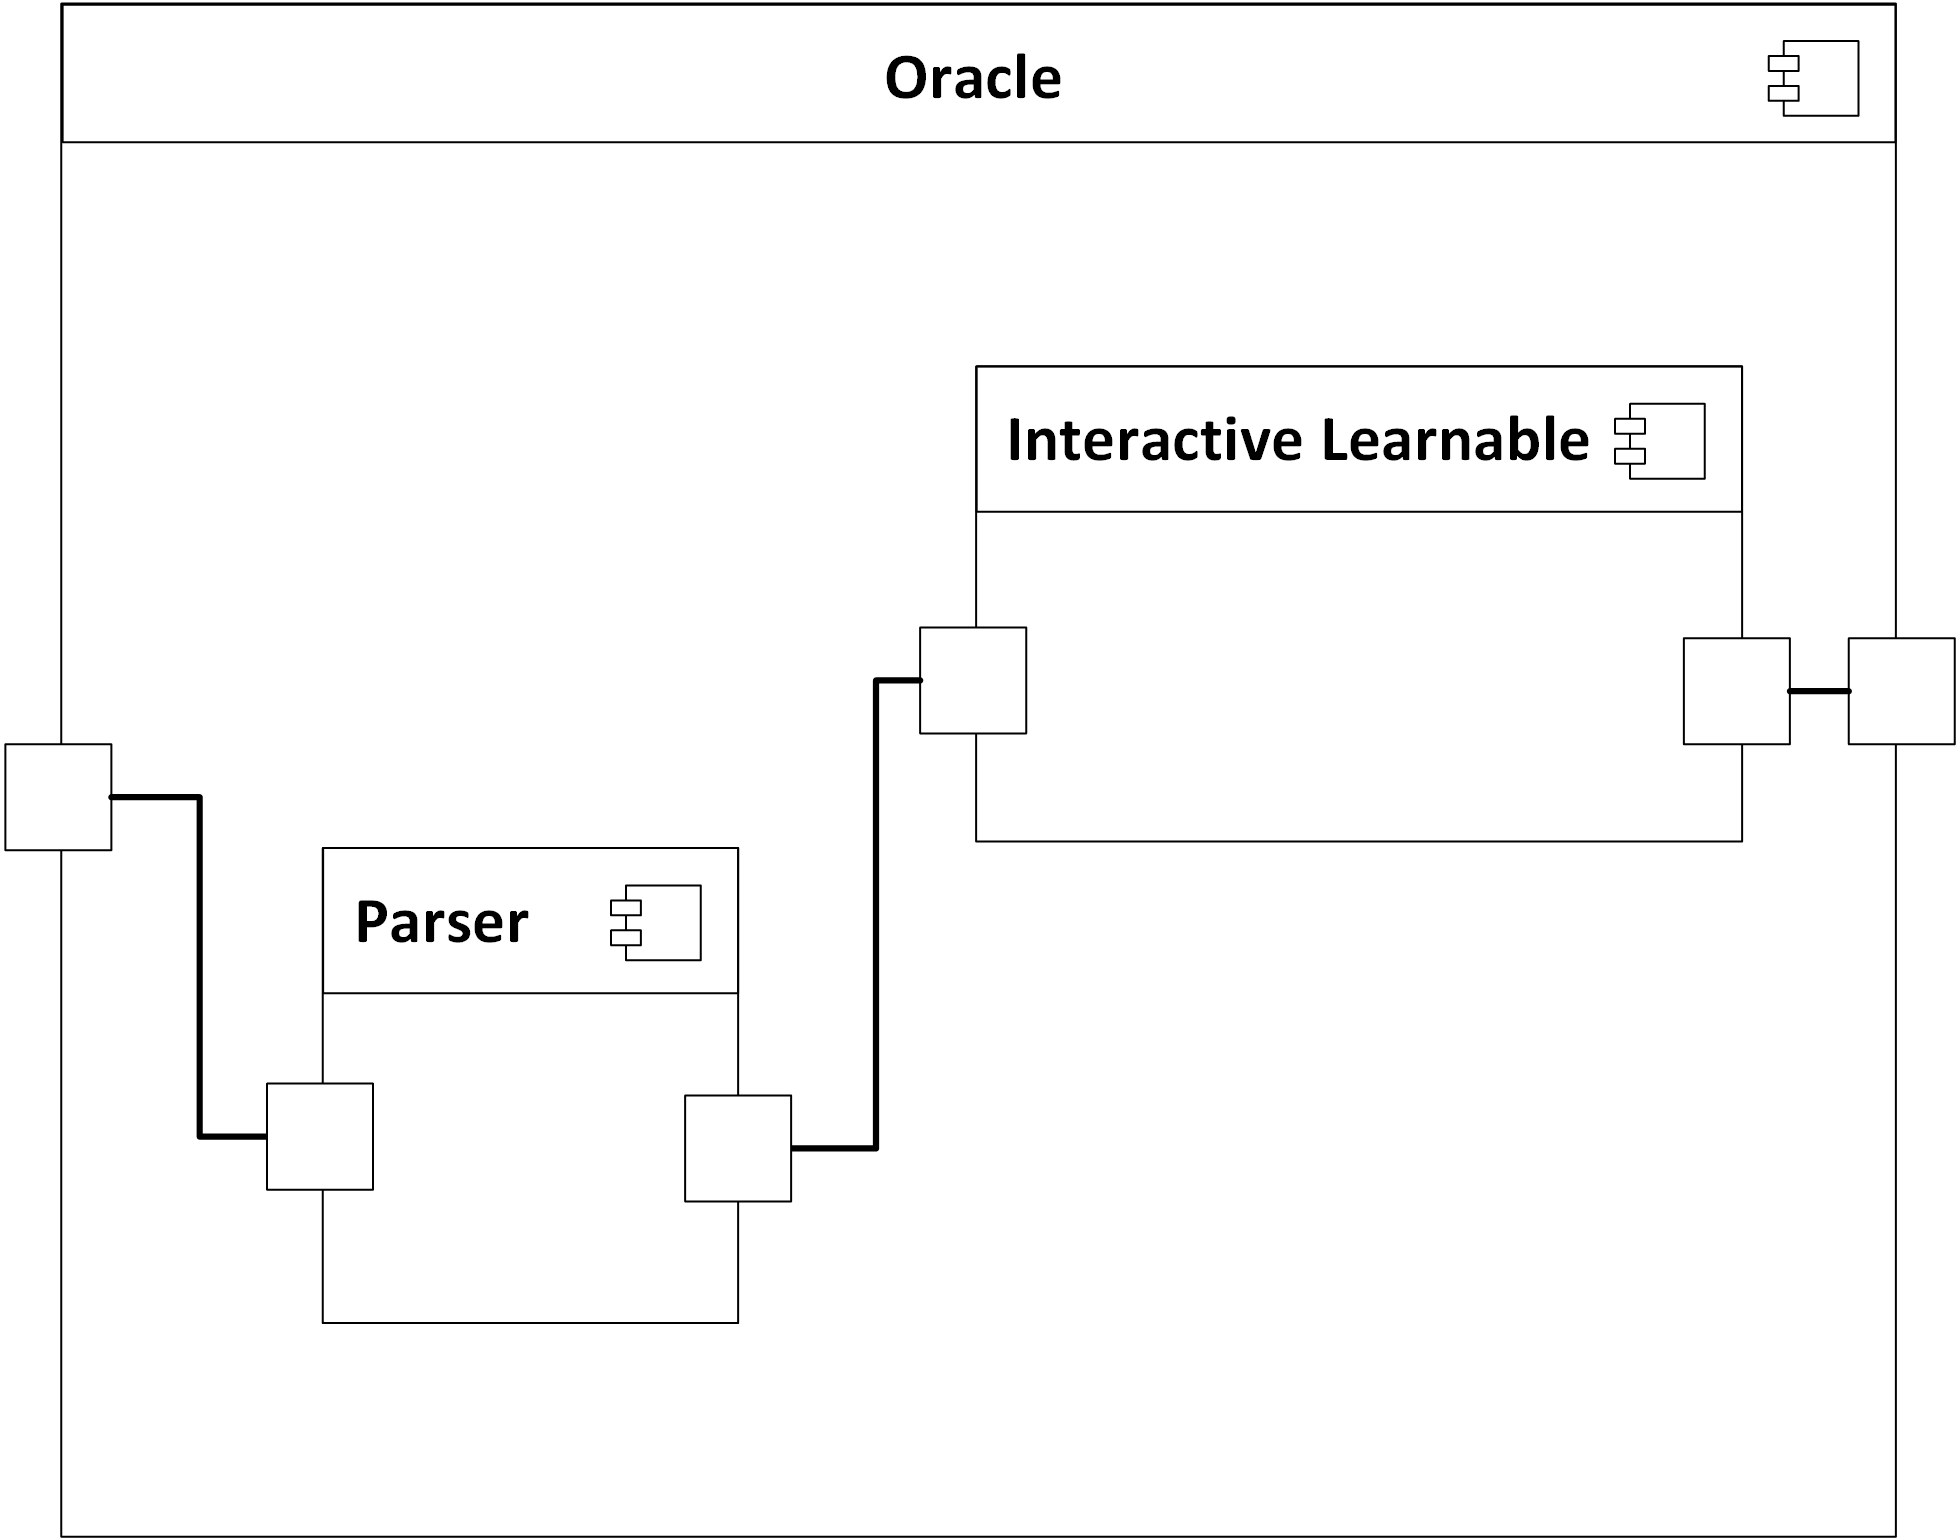
\includegraphics[width=75mm, keepaspectratio]{figures/architecture_oracle.png}
	%}
	\caption{Architecture of the Oracle} 
	\label{fig_architcture_oracle}
\end{figure}

The oracle is responsible for interacting with the user, managing the provided requirements and extracting information based on the queries posed by the learning algorithm. It consists of two main components: the parser and the interactive learnable.

\textbf{The parser} is responsible for handling the input of the user and transforming it to a formalism interpretable by the interactive learnable. This is necessary for enabling event semantics in requirements, separating the input formalism from that of the possible dependencies, and enabling feedback on the input of the user. This is realized through the conventional architecture of compilers: creating a language for the requirements, generating a parser which creates an abstract syntax tree, then a DOM (Document Object Model) from the input and provides feedback, applying M2M or M2T transformations to the desired formalisms.

\textbf{The interactive learnable} stores the requirements received from the parser in the form of \textit{partial models} and answers the queries of the learning algorithm. The architecture of of the interactive learnable can be seen on Figure \ref{fig_architcture_interactivelearnable}.

\begin{figure}[!ht] 
	\centering
	%\fbox{
	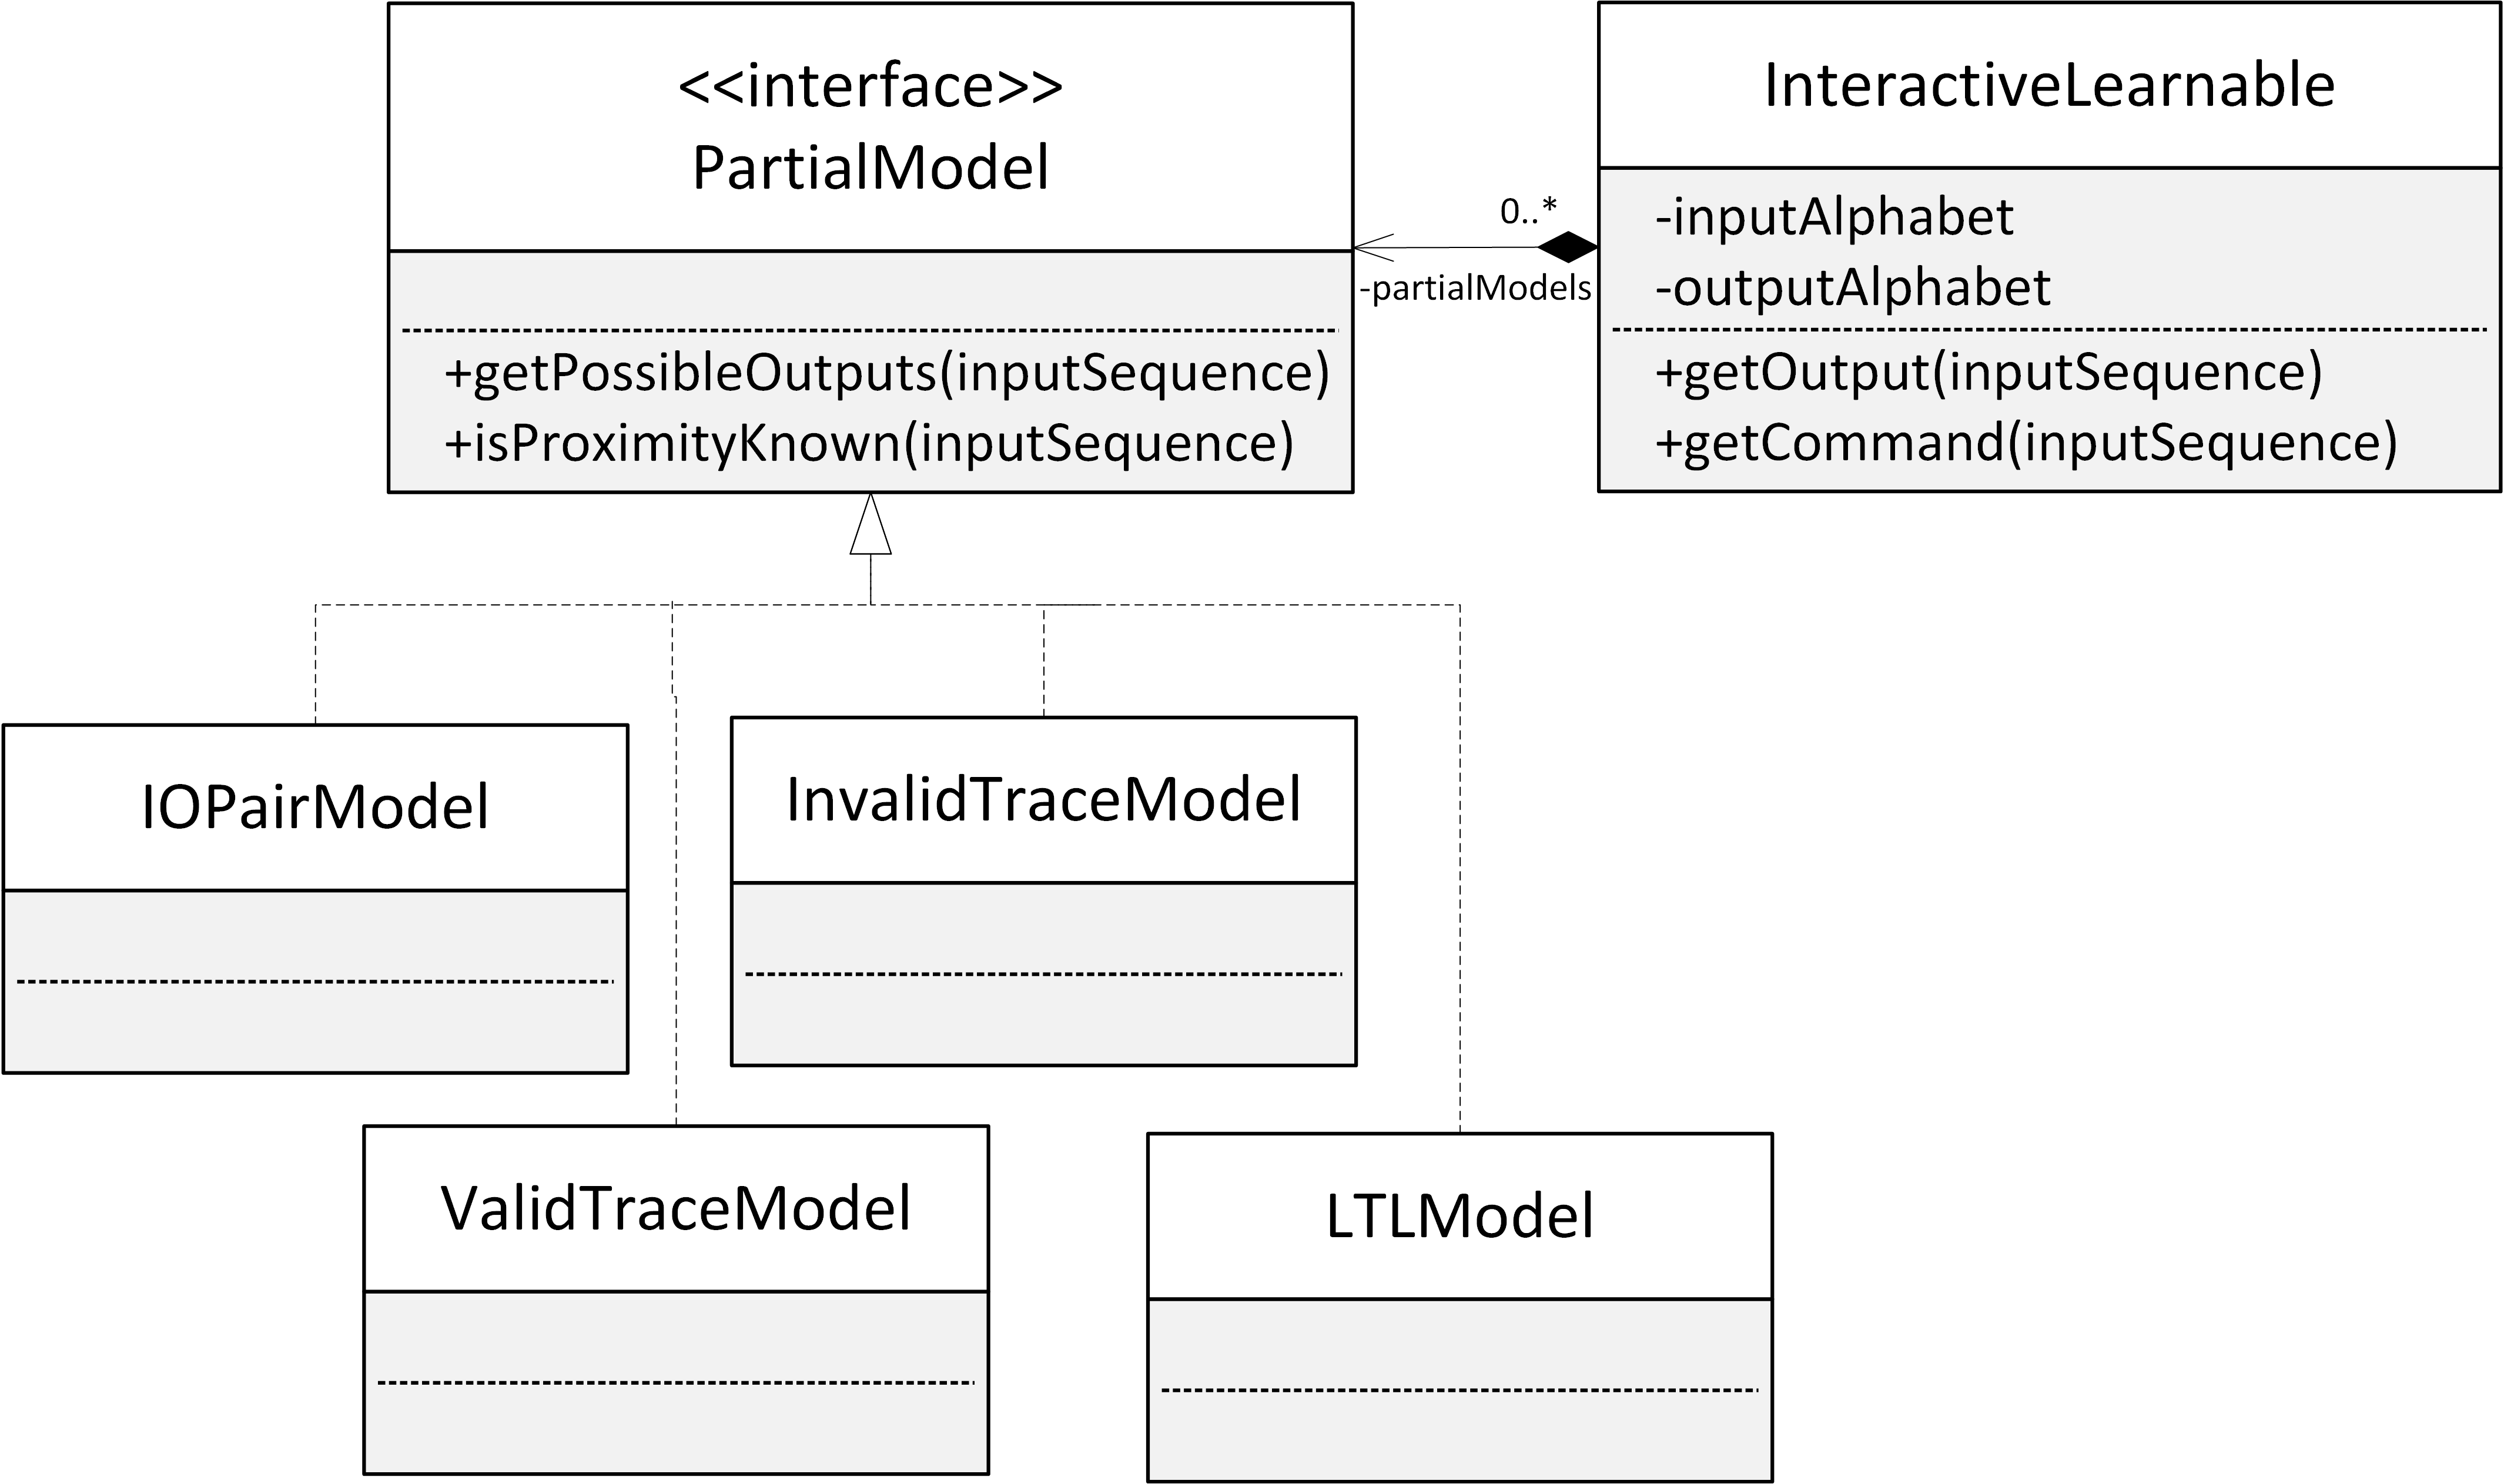
\includegraphics[width=100mm, keepaspectratio]{figures/architecture_interactivelearnable.png}
	%}
	\caption{Architecture of the interactive learnable component} 
	\label{fig_architcture_interactivelearnable}
\end{figure}

Partial models have two responsibilities: providing the set of possible outputs to the given input sequences based on the information contained within, and providing information about the proximity of the input sequence. The intersection of these possible outputs provides the output based on the given requirements, and also reveals conflicting requirements without additional overhead. In the current approach, the inconclusive outputs are delegated to the user, creating the loop on Figure \ref{fig_providerequirementsworkflow}.

Telling whether partial models contain additional information enables the interactive learnable to track the easly explorable parts of the design space, thus facilitating significant optimization opportunities for the entire workflow through attaching one of the proposed adaption commands to the answer to each query. For instance, when a given valid trace is queried for an output somewhere in the middle of its contained sequence, the exploration of the rest of its contained behaviors can be automatically queried without requiring the input of the user. 

Preserving the requirements in separate partial models has several advantages. First of all, it ensures the traceability between the user input and the learning algorithm, which is essential, as the user may not understand feedback or questions about information derived from their input. Also, translating each requirement to a common formalism and merging these models might be possible, but the addition and removal of models - which is a frequent operation in the workflow - would be severely ineffective. Additionally, in this manner the exploration of the individual models may be adjusted to their own internal logic.

Supporting model conflict handling -- as proposed in Subsection \ref{subs_conf} -- introduces two serious problems: models have to be able to be removed just as easily as they can be added, and inconsistencies need to be handled when removing a model. The first problem is solved by our partial model pattern, but the other one requires further consideration. Model inconsistency arises, when a model has been used to answer behavior-related queries, then it is removed. In this case, the already extracted information remains in the system, but its source disappears. Our solution to this problem, is to restart the automata learning -- retaining the models already provided by the user, thus hiding this restart -- by attaching a $RESET$ command to the answer to the queries of the adaptive learning algorithm.

Currently, there are two main types of partial models - corresponding to the two main types of requirements: trace-based models, which store valid or invalid scenarios for an execution of a model, and LTL models, containing high-level behavioral properties which must be fulfilled by the resulting model. The following two subsections elaborate on these models. 

%---------------------------------------------------------------
%\subsection{Trace-Based Models} \label{subs_traceintheframework}
%---------------------------------------------------------------

\textbf{Trace-based models} correspond to trace-based requirements and store a arbitrarily long finite sequence of input-output pairs. The corresponding requirement types include: corresponding outputs to input sequences, valid and invalid traces and sequence diagrams. 

The common property of these models is that they can be represented via conventional incomplete finite automata. The automata contain information about a given input sequence if they reach an accepting state at the end of the word. They contain more information when other accepting states are reachable from that point.

Trace-based requirement types are mapped to a specific kind of partial model representing the corresponding automaton. Although each of these automata is a finite automaton, they vary greatly in their complexity of execution, thus the complexity of their provided behavior. The number of these models can be huge with very frequent execution.

For instance, in case of IOPairModels (corresponding output-type requirements), it is enough to check if the accepting state can be reached and they surely contain no additional information. However, sequence diagrams can contain branching and loops in the behavior, thus require more complex algorithms.

%\begin{figure}[!ht] 
%	\centering
%	\fbox{
%		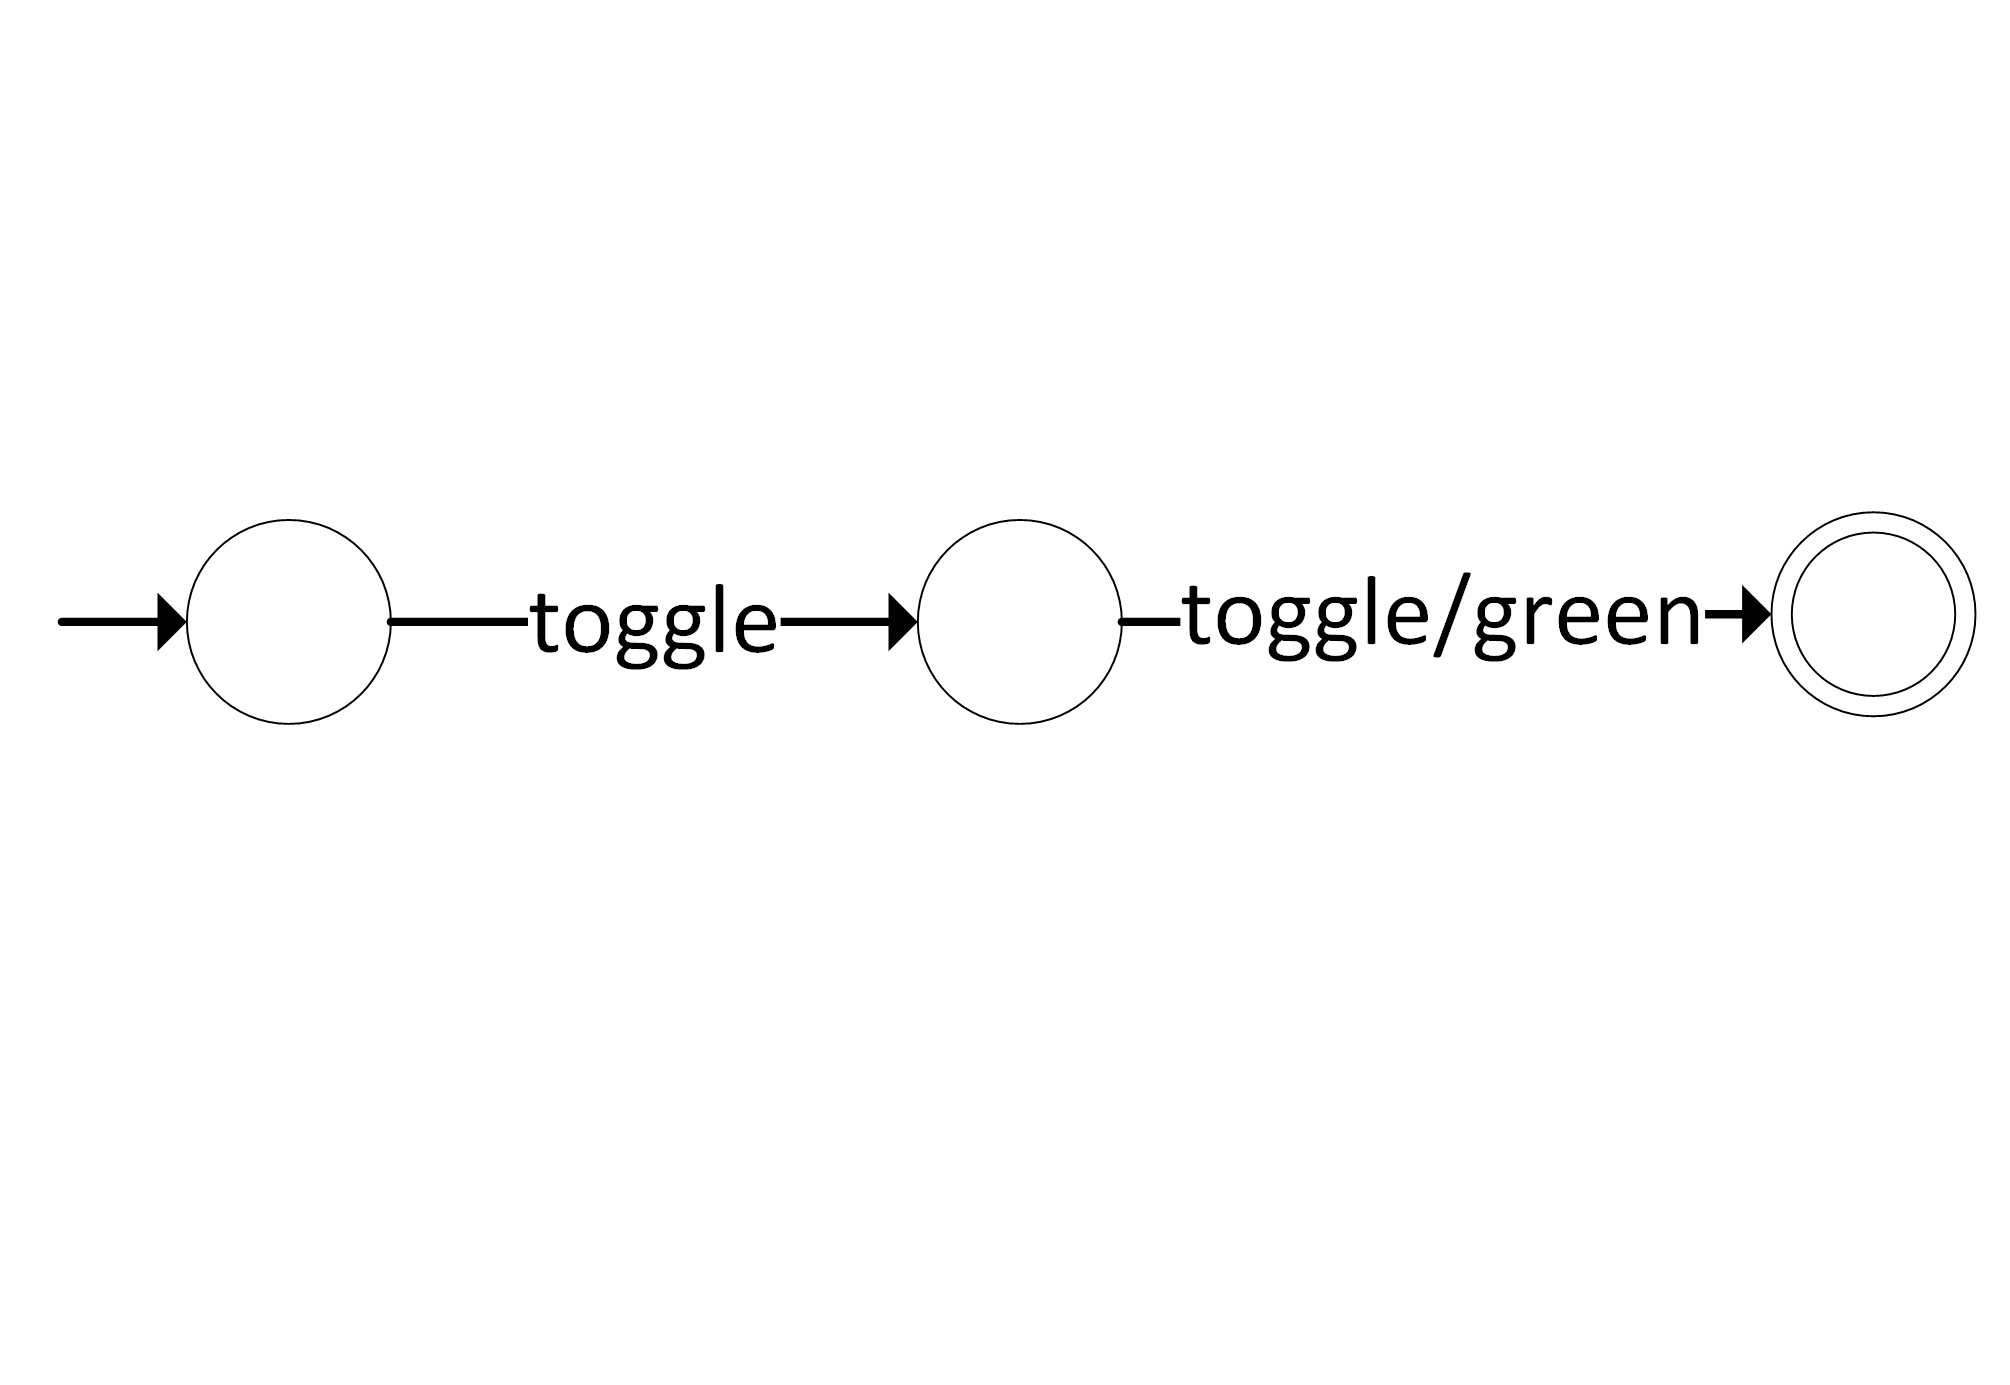
\includegraphics[width=40mm, keepaspectratio]{figures/architecture_iopairautomaton.png}
%	}
%	\fbox{
%		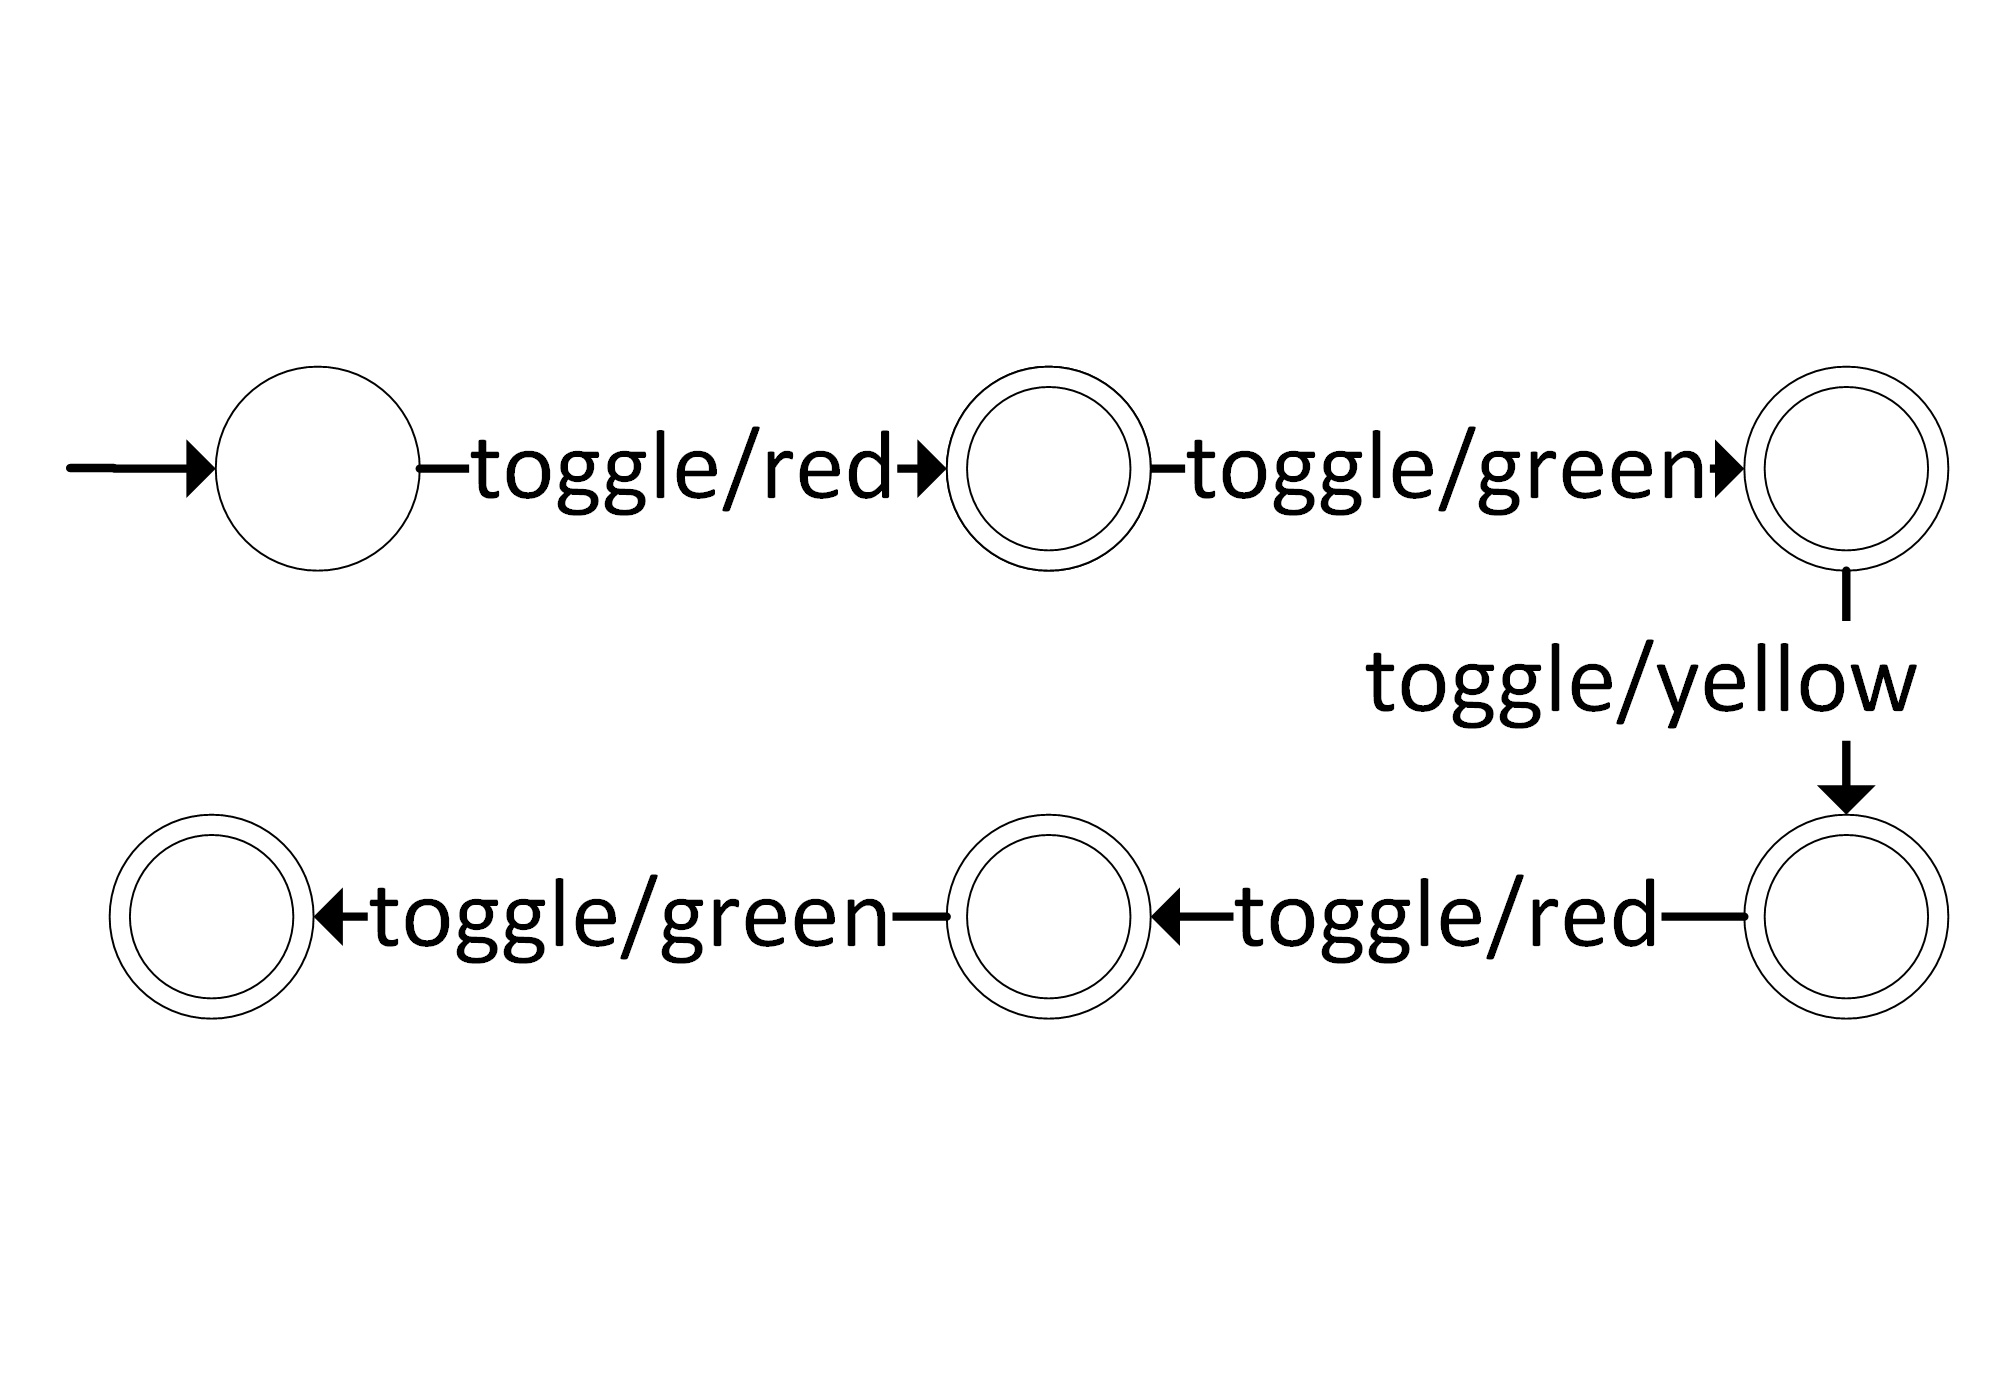
\includegraphics[width=40mm, keepaspectratio]{figures/architecture_traceautomaton.png}
%	}
%	\fbox{
%		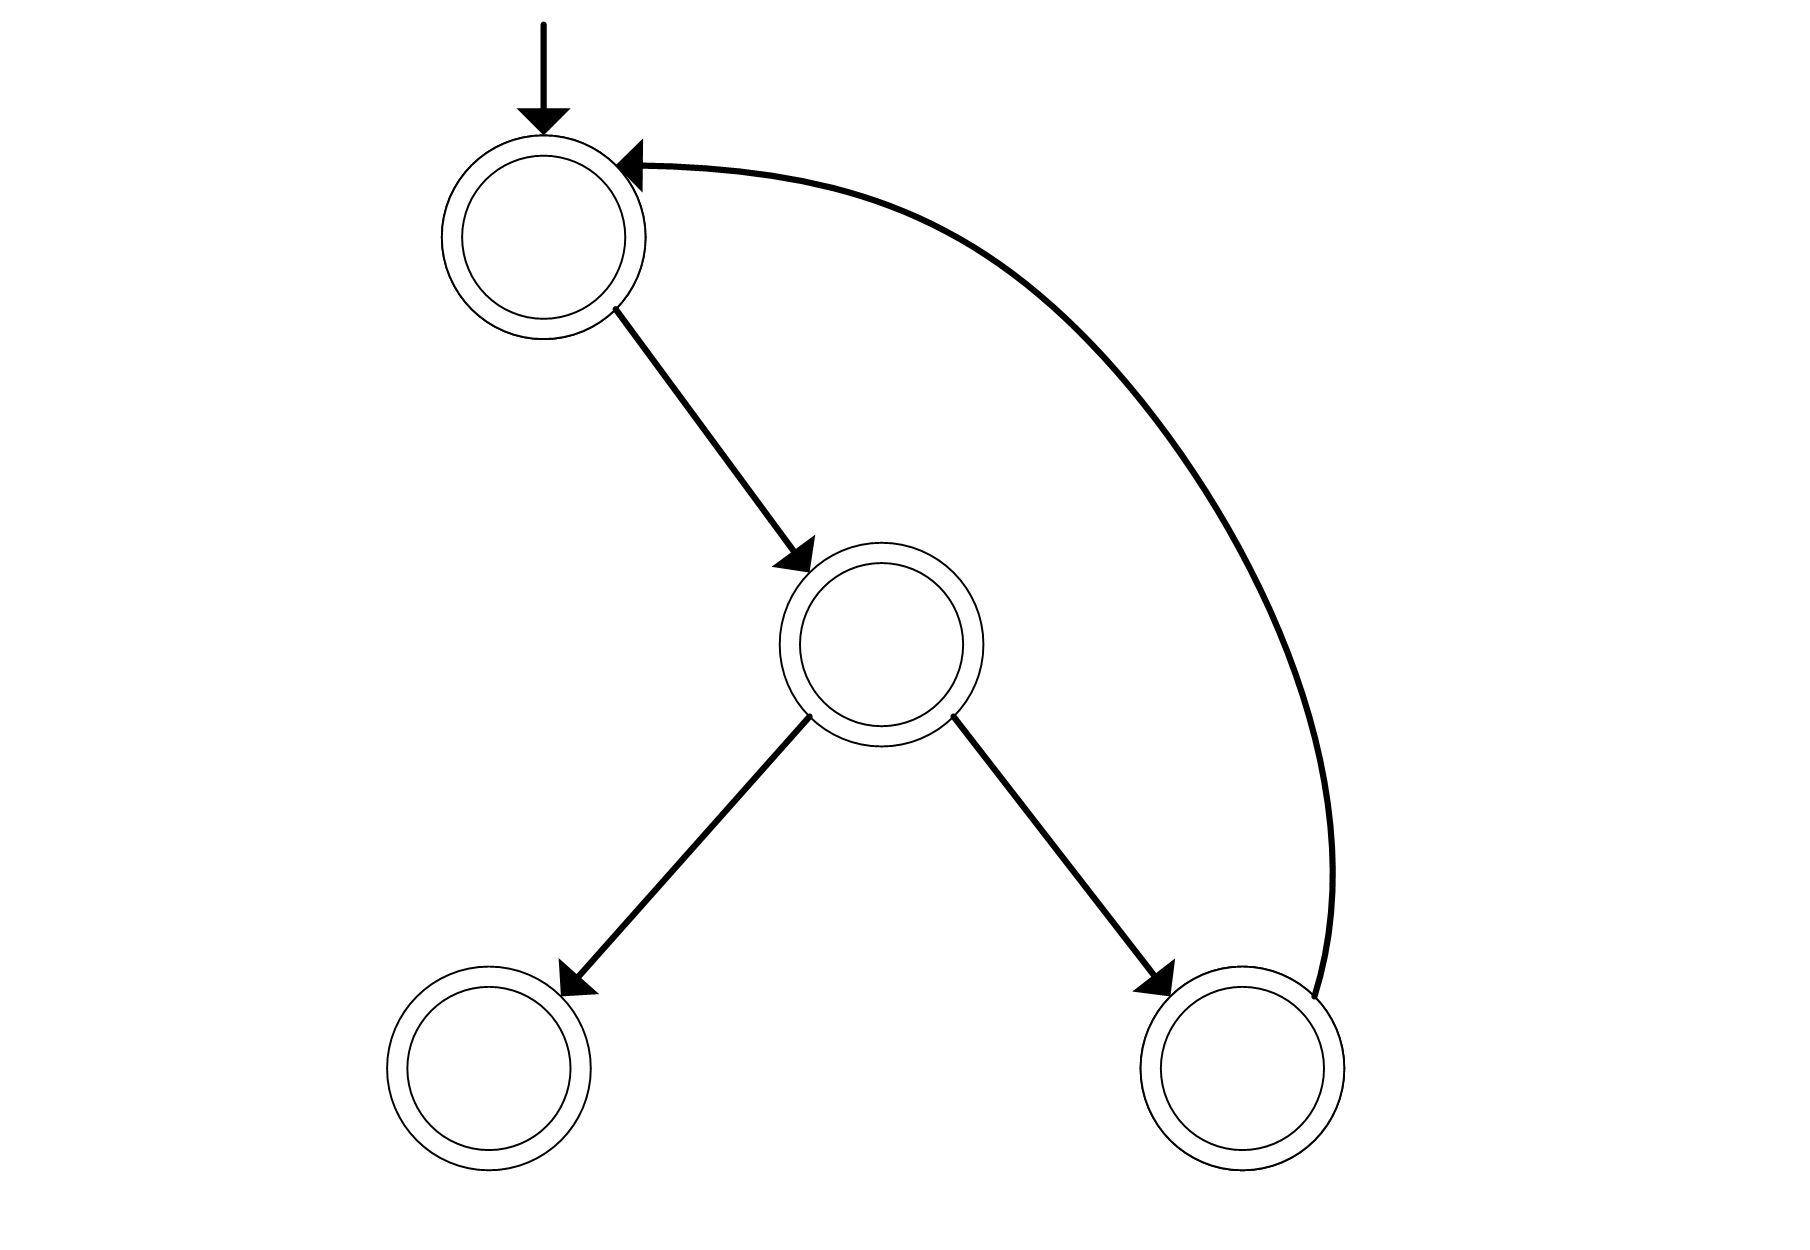
\includegraphics[width=40mm, keepaspectratio]{figures/architecture_sequenceautomaton.png}
%	}
%	\caption{Characteristic automaton types of the different requirements: corresponding output (\textit{left}), valid trace (\textit{middle}) and sequence diagram (\textit{right})} 
%	\label{fig_architcture_traceautomata}
%\end{figure}

%---------------------------------------------------------------
%\subsection{LTL Models} \label{subs_ltlintheframework}
%---------------------------------------------------------------

\textbf{LTL models} on the other hand correspond to LTL requirements: program logic based requirements that describe the behavior for infinite input/output sequences.%: $\omega$-regular languages.

They correspond to nondeterministic $\omega$-automata. As the acceptance condition of Büchi-automata is closest to that of finite automata -- as shown in Chapter \ref{background} --, we chose them for the target of the mapping of the corresponding requirements. It should be noted, that any of the automata classes recognizing the $\omega$-regular languages could have been chosen with an appropriate interpretation.

As Büchi automata accept only infinitely long words over the given input alphabet, the process of the determination of the possible outputs - the condition of a character being marked a possible output - was adopted accordingly.

In our interpretation, a Büchi automaton has information about a given finite input sequence, if at the end of the input the automaton reaches an accepting state. Then the possible outputs are the elements of the output alphabet on the last edge taken. As the automaton is nondeterministic (and cannot be determinized), there may be multiple accepting states, thus multiple edges, and even one edge might contain multiple possible outputs. In this case the conjunction of the possible outputs on the corresponding edges is the possible output of the automaton.  

There may be other interpretations of Büchi automata in this context. For instance, it would be enough for an input sequence to reach a state from which an accepting state is reachable. This would provide an answer in more cases, than our interpretation, but also introduce faulty behavior which would have to be handled in the workflow. Also, it would be possible to track impossible outputs when no accepting state can be reached.

A summarizing example of the different automaton types can be seen on figure \ref{fig_architecture_buchiexample}.

\begin{figure}[!ht] 
	\centering
	\fbox{
		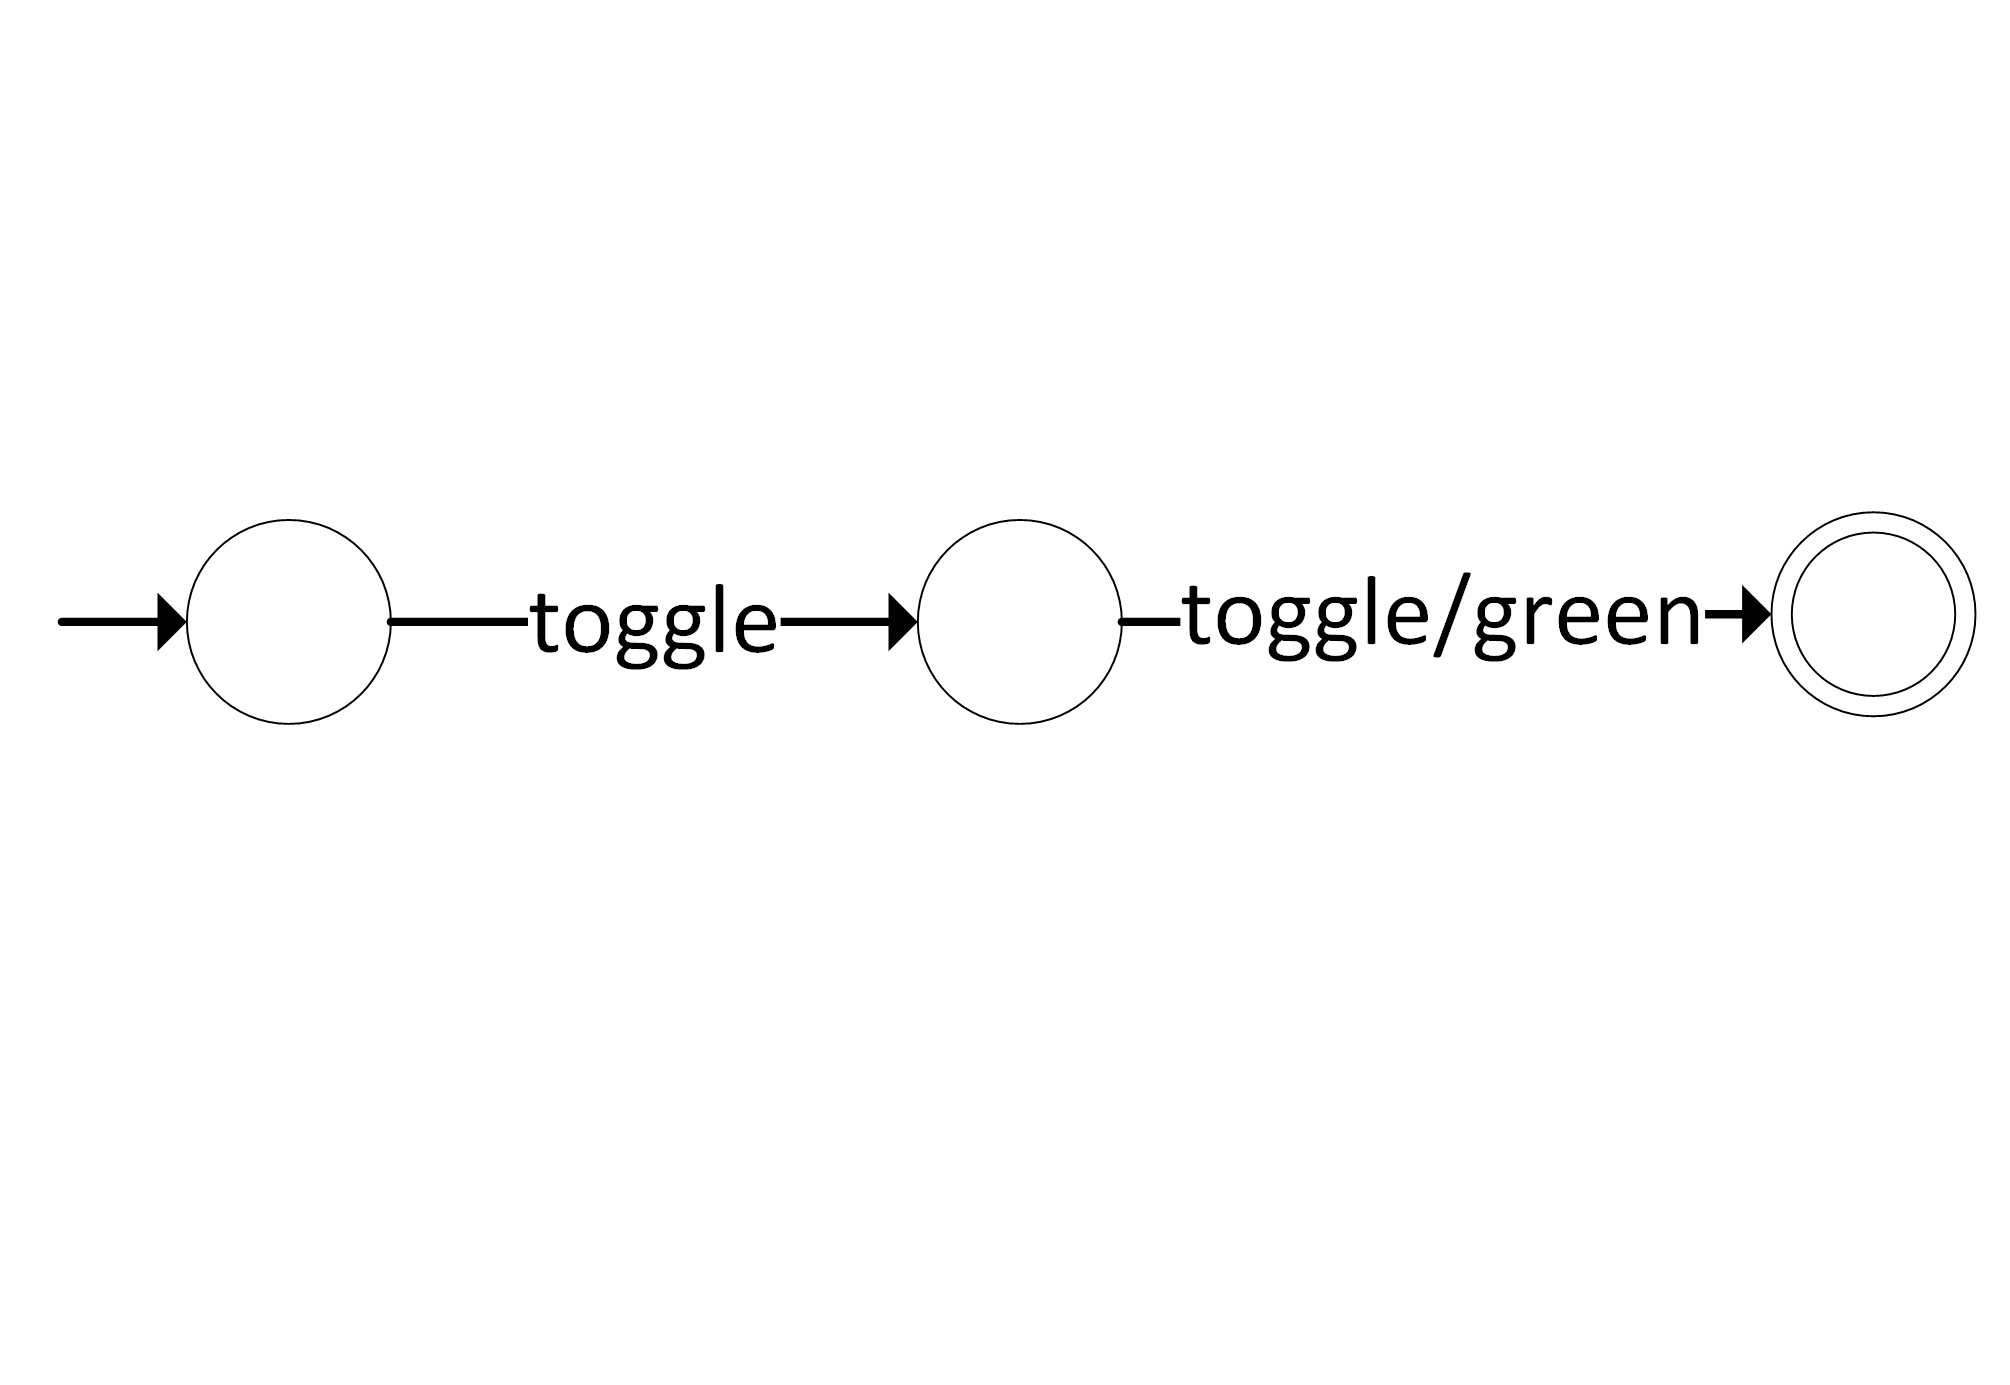
\includegraphics[width=60mm, keepaspectratio]{figures/architecture_iopairautomaton.png}
	}
	\fbox{
		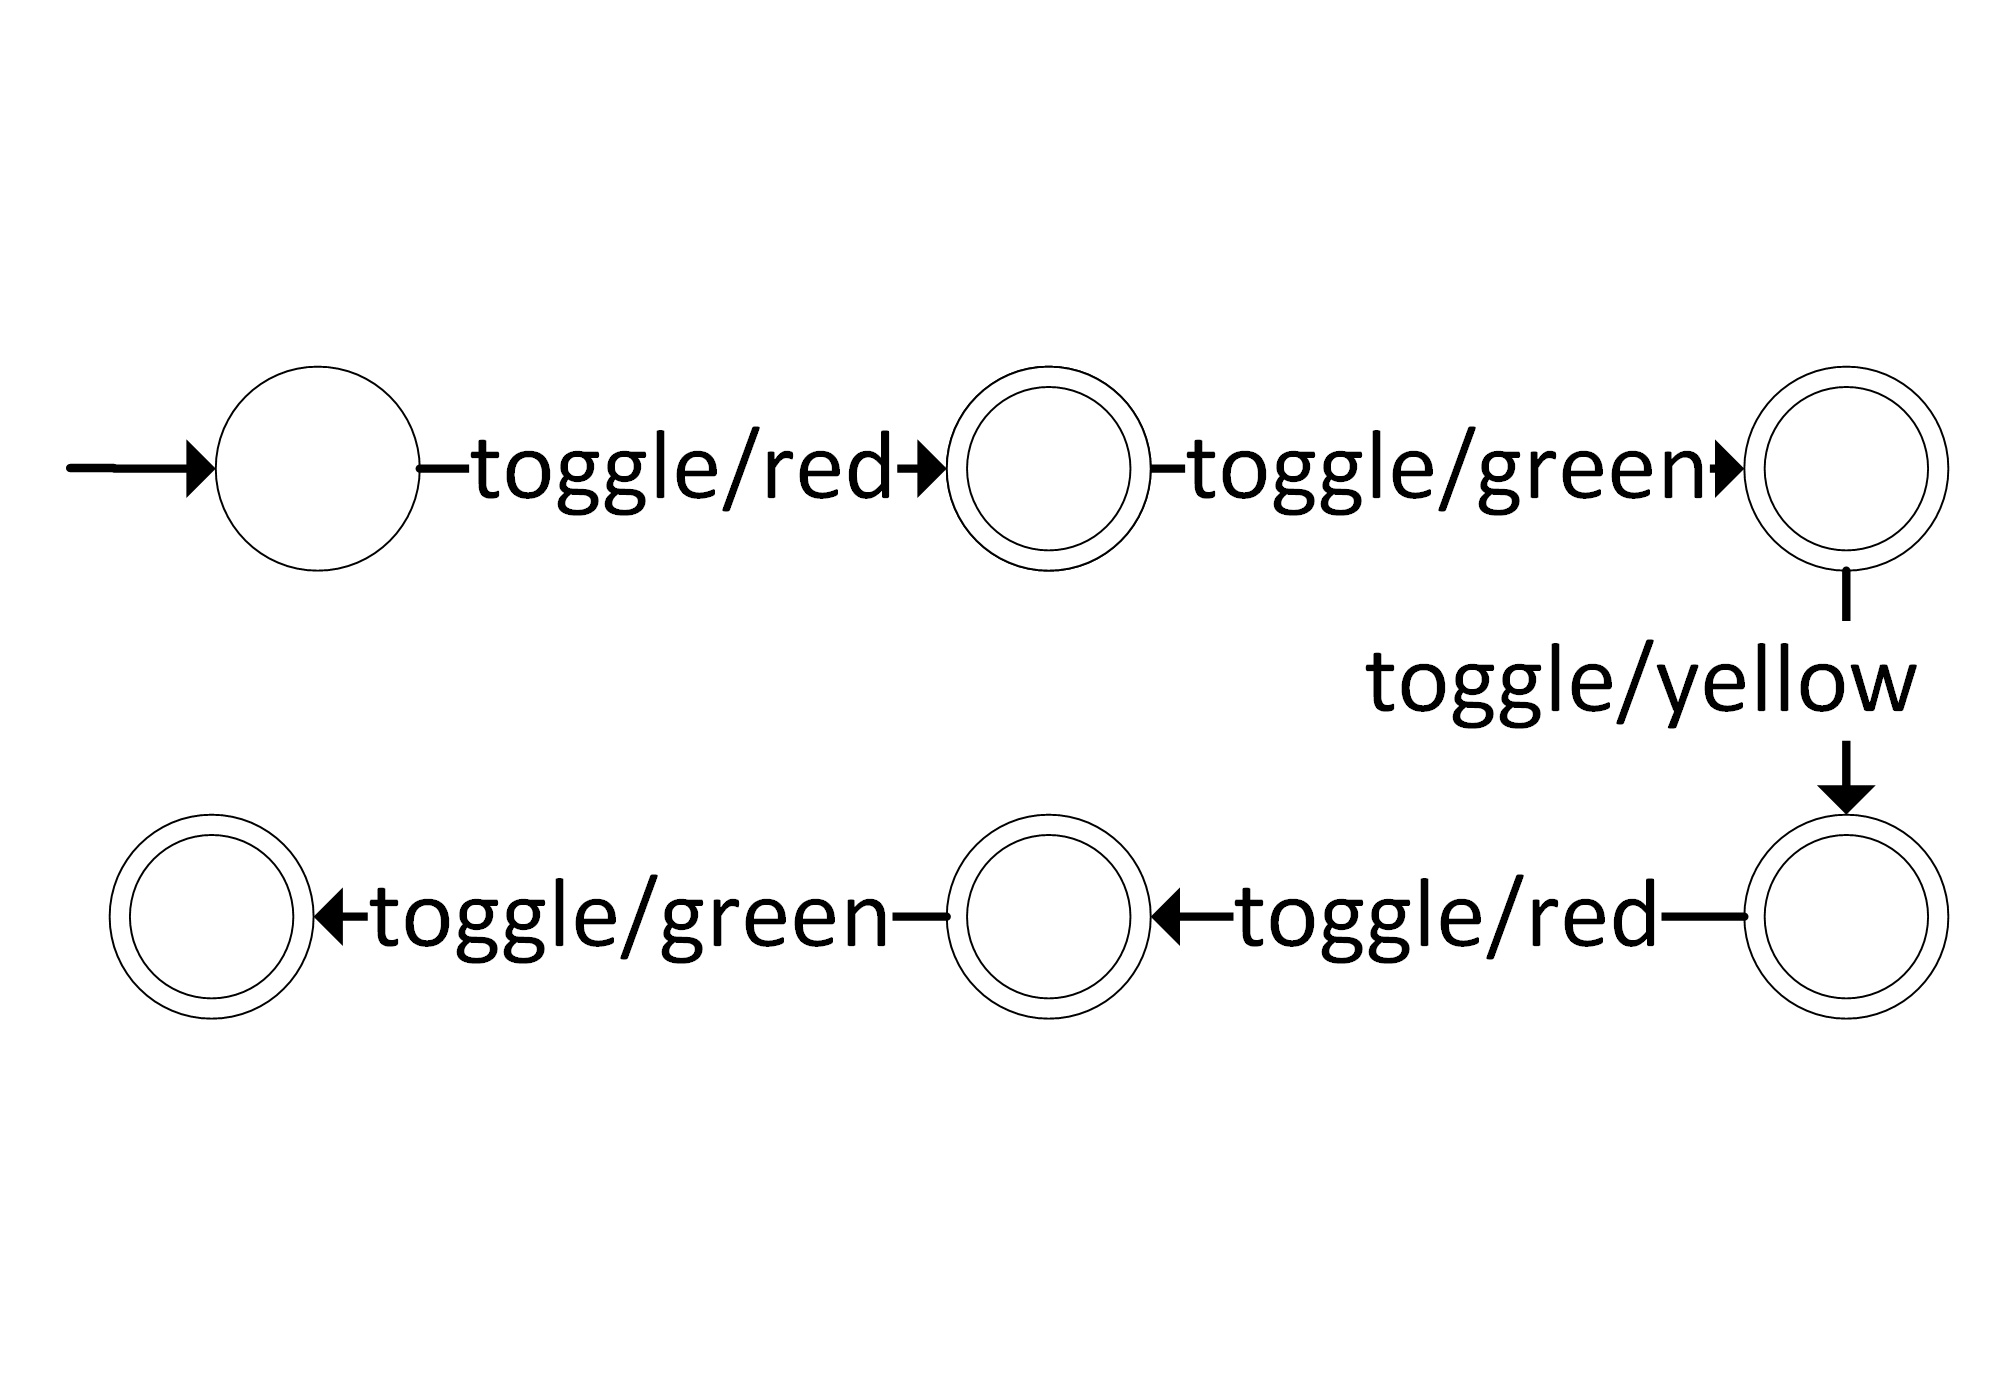
\includegraphics[width=60mm, keepaspectratio]{figures/architecture_traceautomaton.png}
	}
	\fbox{
		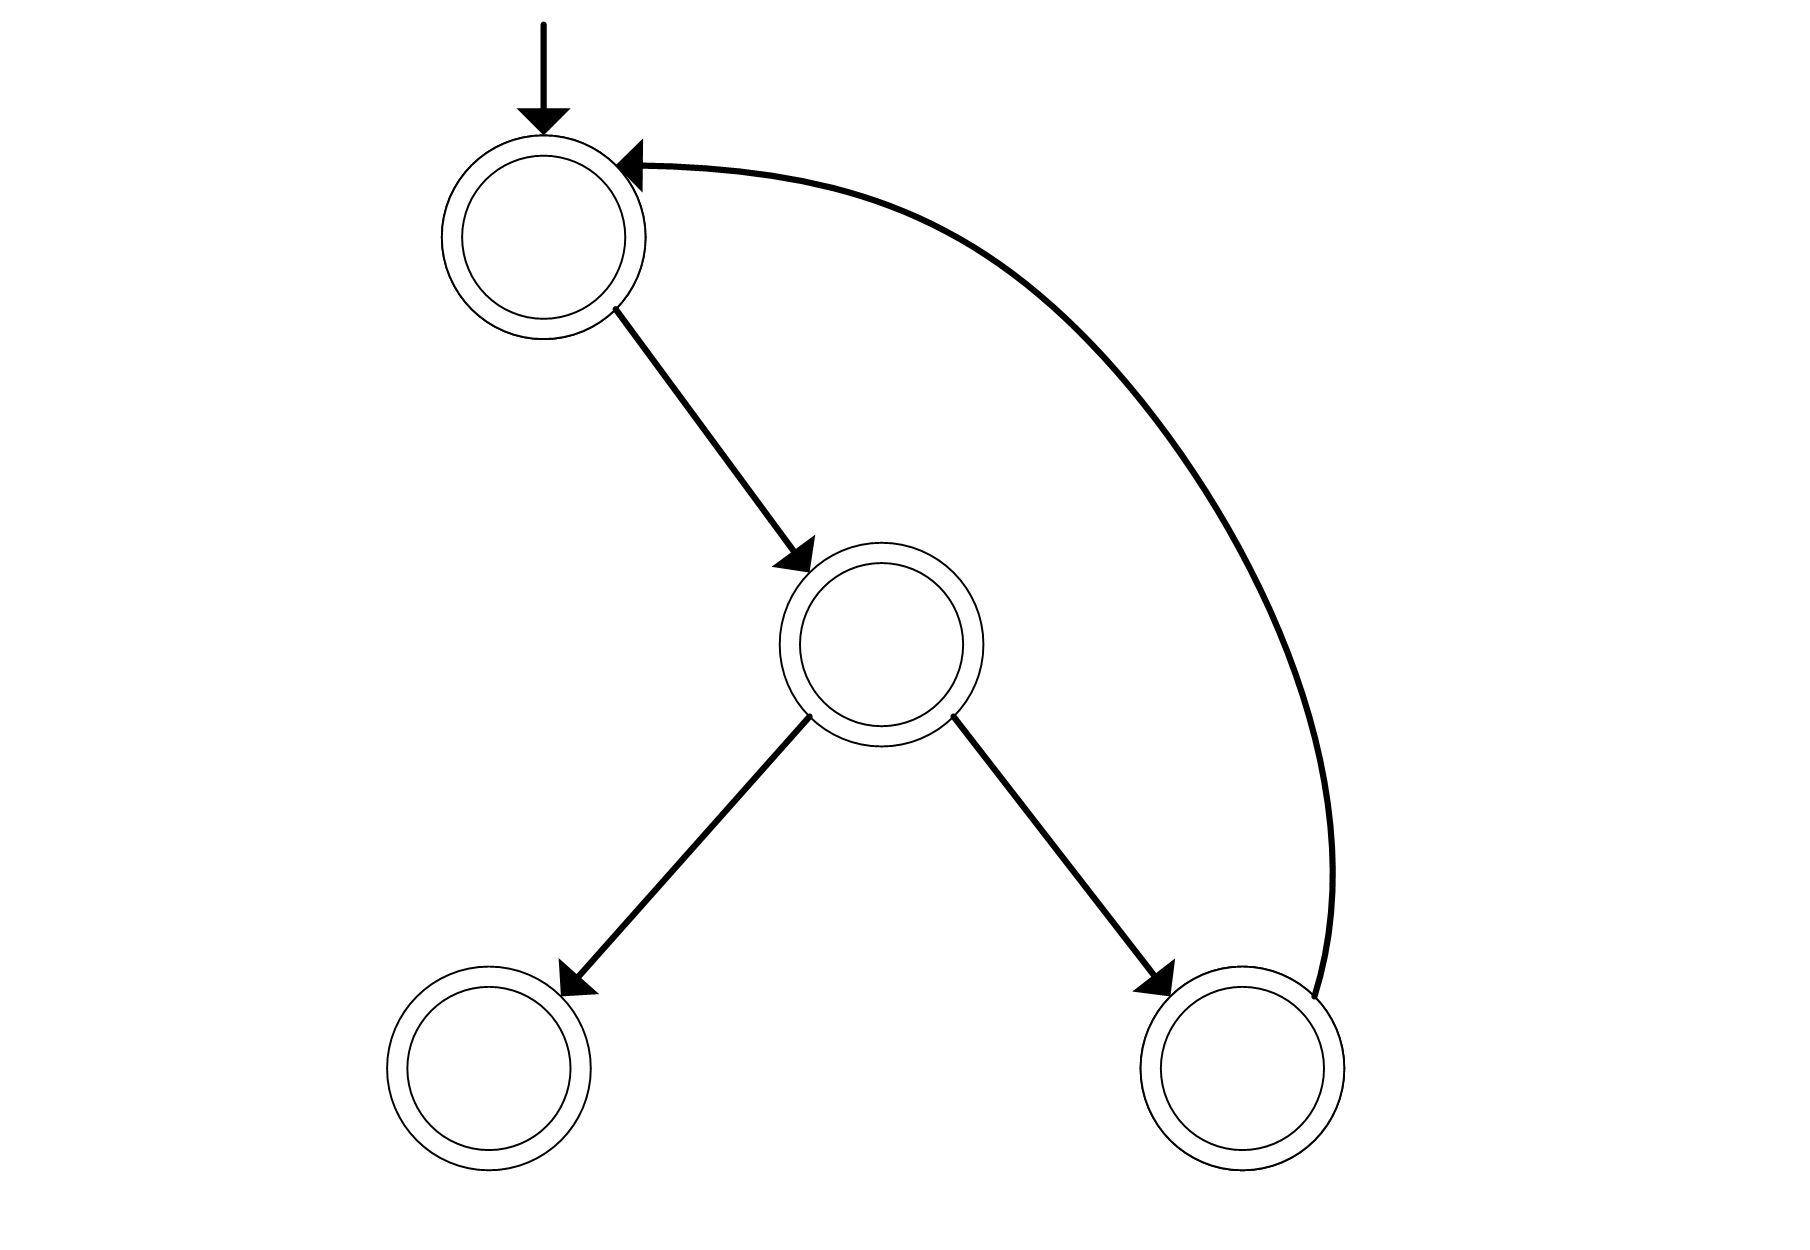
\includegraphics[width=60mm, keepaspectratio]{figures/architecture_sequenceautomaton.png}
	}
	\fbox{
		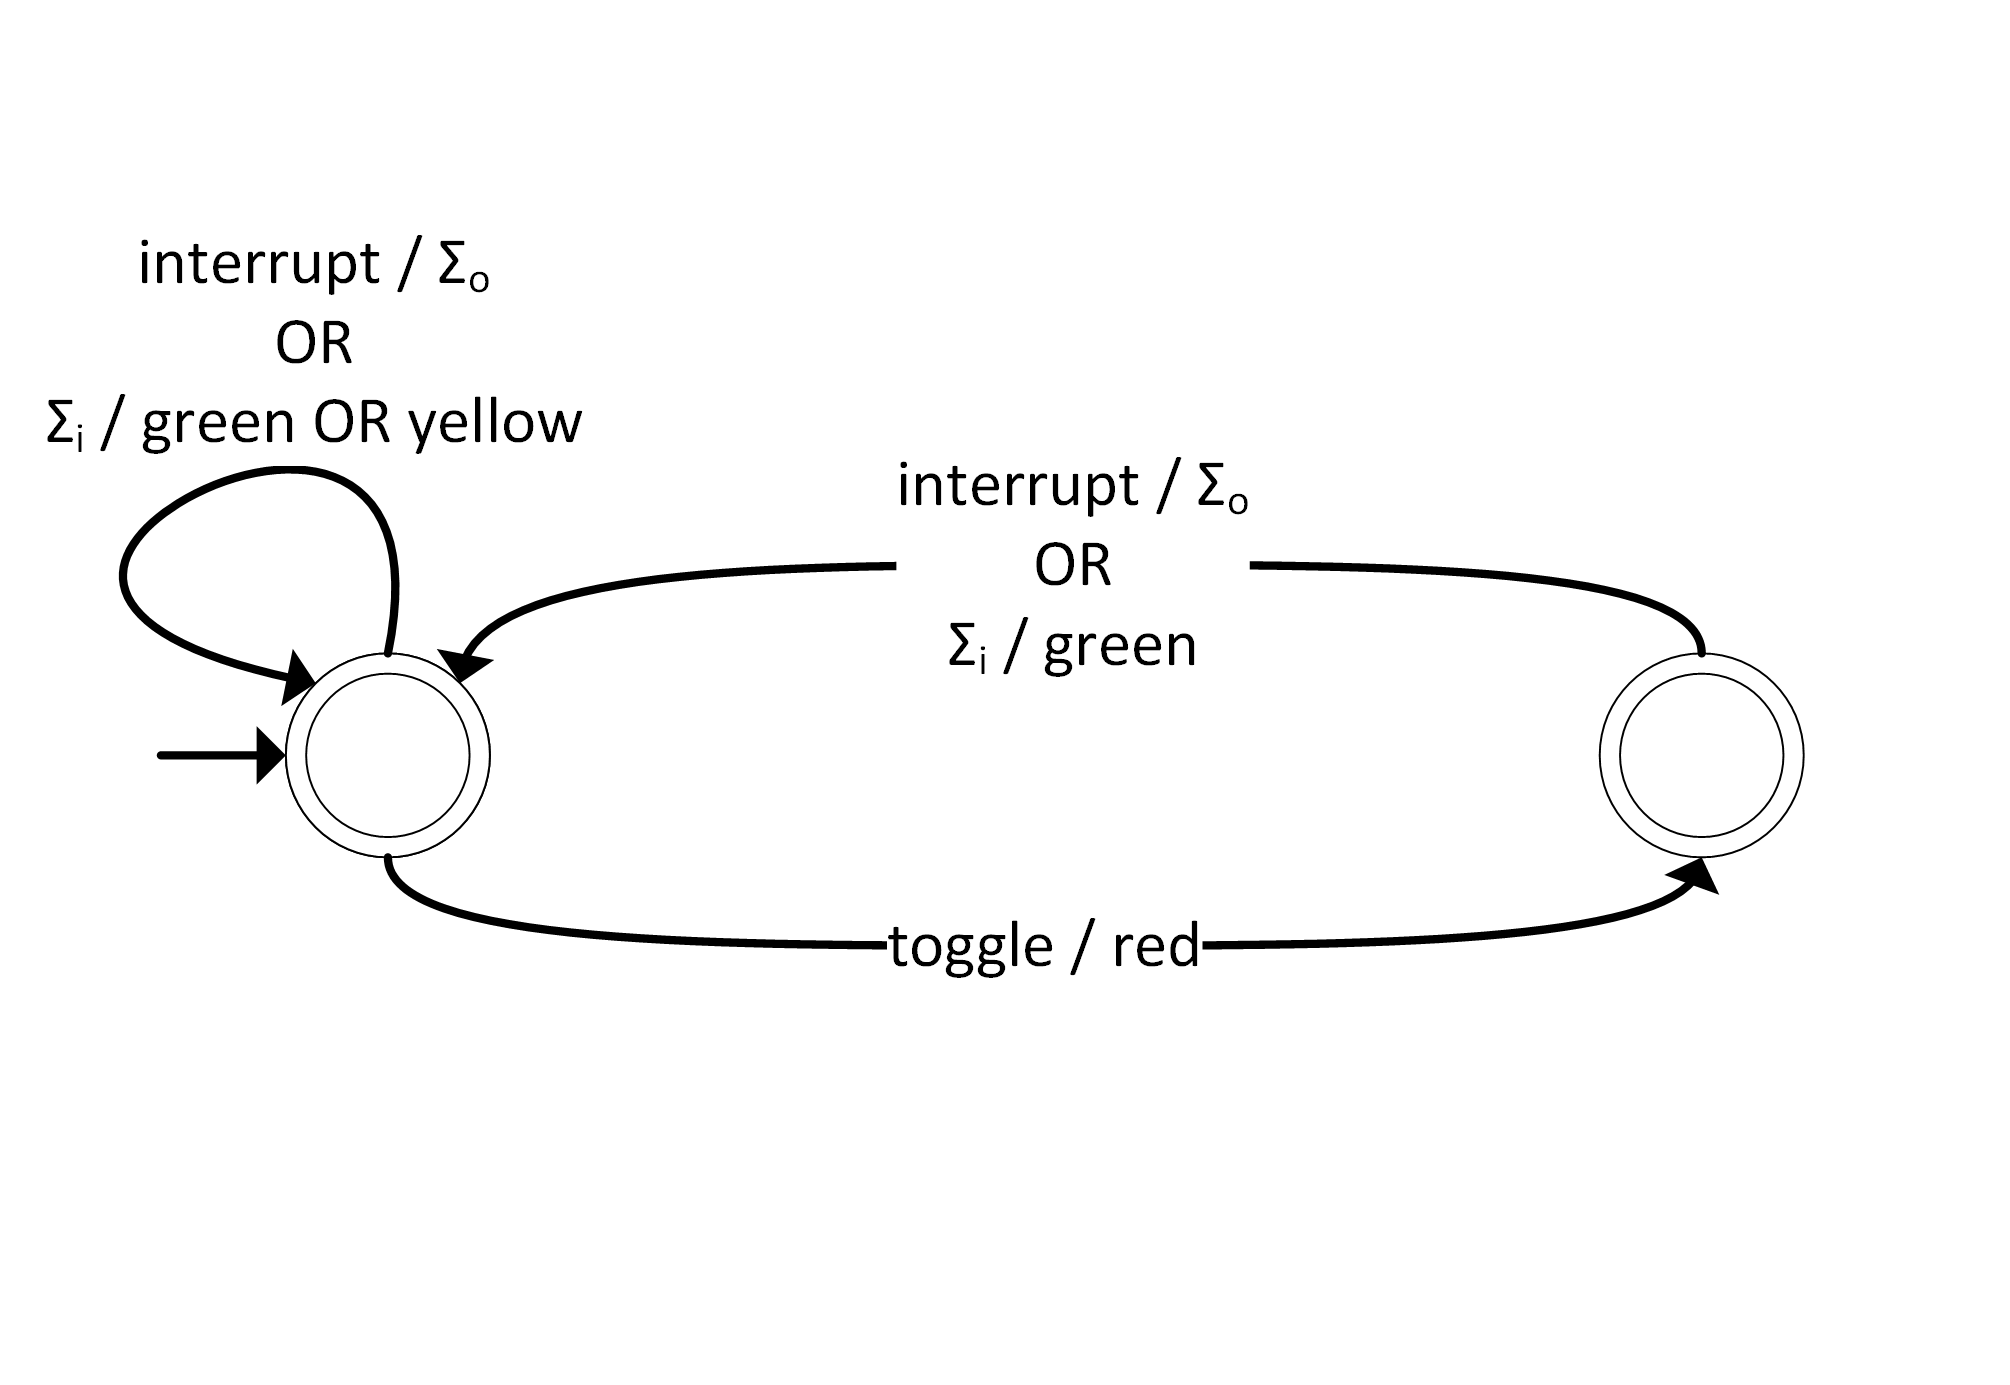
\includegraphics[width=60mm, keepaspectratio]{figures/architecture_buchiexample.PNG}
	}
	\caption{Examples for attempting to model the requirement 'after toggle/red, for toggle the output is green' through I/O pair automaton (\textit{upper left}), valid trace automaton (\textit{upper right}), sequence diagram automaton (\textit{lower left}) and a Büchi automaton (\textit{lower right}).} 
	\label{fig_architecture_buchiexample}
\end{figure}

%---------------------------------------------------------------
\subsection{The Learning Algorithm} \label{subs_dhcintheframework}
%---------------------------------------------------------------

There are a variety of approaches to active automata learning, differing in the number of queries and the logical order in which they are asked. To fully utilize the proposed interactive learning, the used automata learning algorithm is required to:

\begin{itemize}
	\item allow the addition, removal and modification of requirements (and thus the learned behavior), and
	\item to be easily extensible and open for modification, such that the adaptive consideration of explorable and inferable behaviors - enabled through the proposed interactive learnable - can be utilized.
\end{itemize}

To support the above requirements, we built upon and designed a variant of the Direct Hypothesis Construction algorithm. The DHC algorithm learns through rounds of hypothesis creation, in which every round starts from the ground-up. This approach has the benefit of allowing the system under learning to behaviorally change through the run of the algorithm, and - in the case of interactive learning - allows the designing engineer(s) to add, remove and modify requirements during the online phase of the workflow. The Direct Hypothesis Construction algorithm is also a straightforward and easily modifiable algorithm, making the adaption to specific heuristics simple to design and implement. In order to make adaption possible, the teacher component of automata learning needs to handle not only the output of a query, but also the adaption heuristic the algorithm should adapt to. This enables an adaptive learning algorithm, which receives both the desired output and the learning heuristic to utilize from its teacher component - keeping an identical, but extended automata learning architecture, as shown in Figure \ref{fig_architcture_learningalgo}. The resulting algorithm can be seen in Algorithm \ref{algo:adaptivedhc}. As \textit{line 7} shows, the membership query returns both the output and the adaption heuristic. If the adaption command is $RESET$, the learning round begins again while keeping the current inputs. The enqueueing of successors is only possible, if the received heuristic is $OPTIMISTIC$, allowing the fine-tuning of exactly which states to explore greedily.

\begin{figure}[!ht] 
	\centering
	%\fbox{
	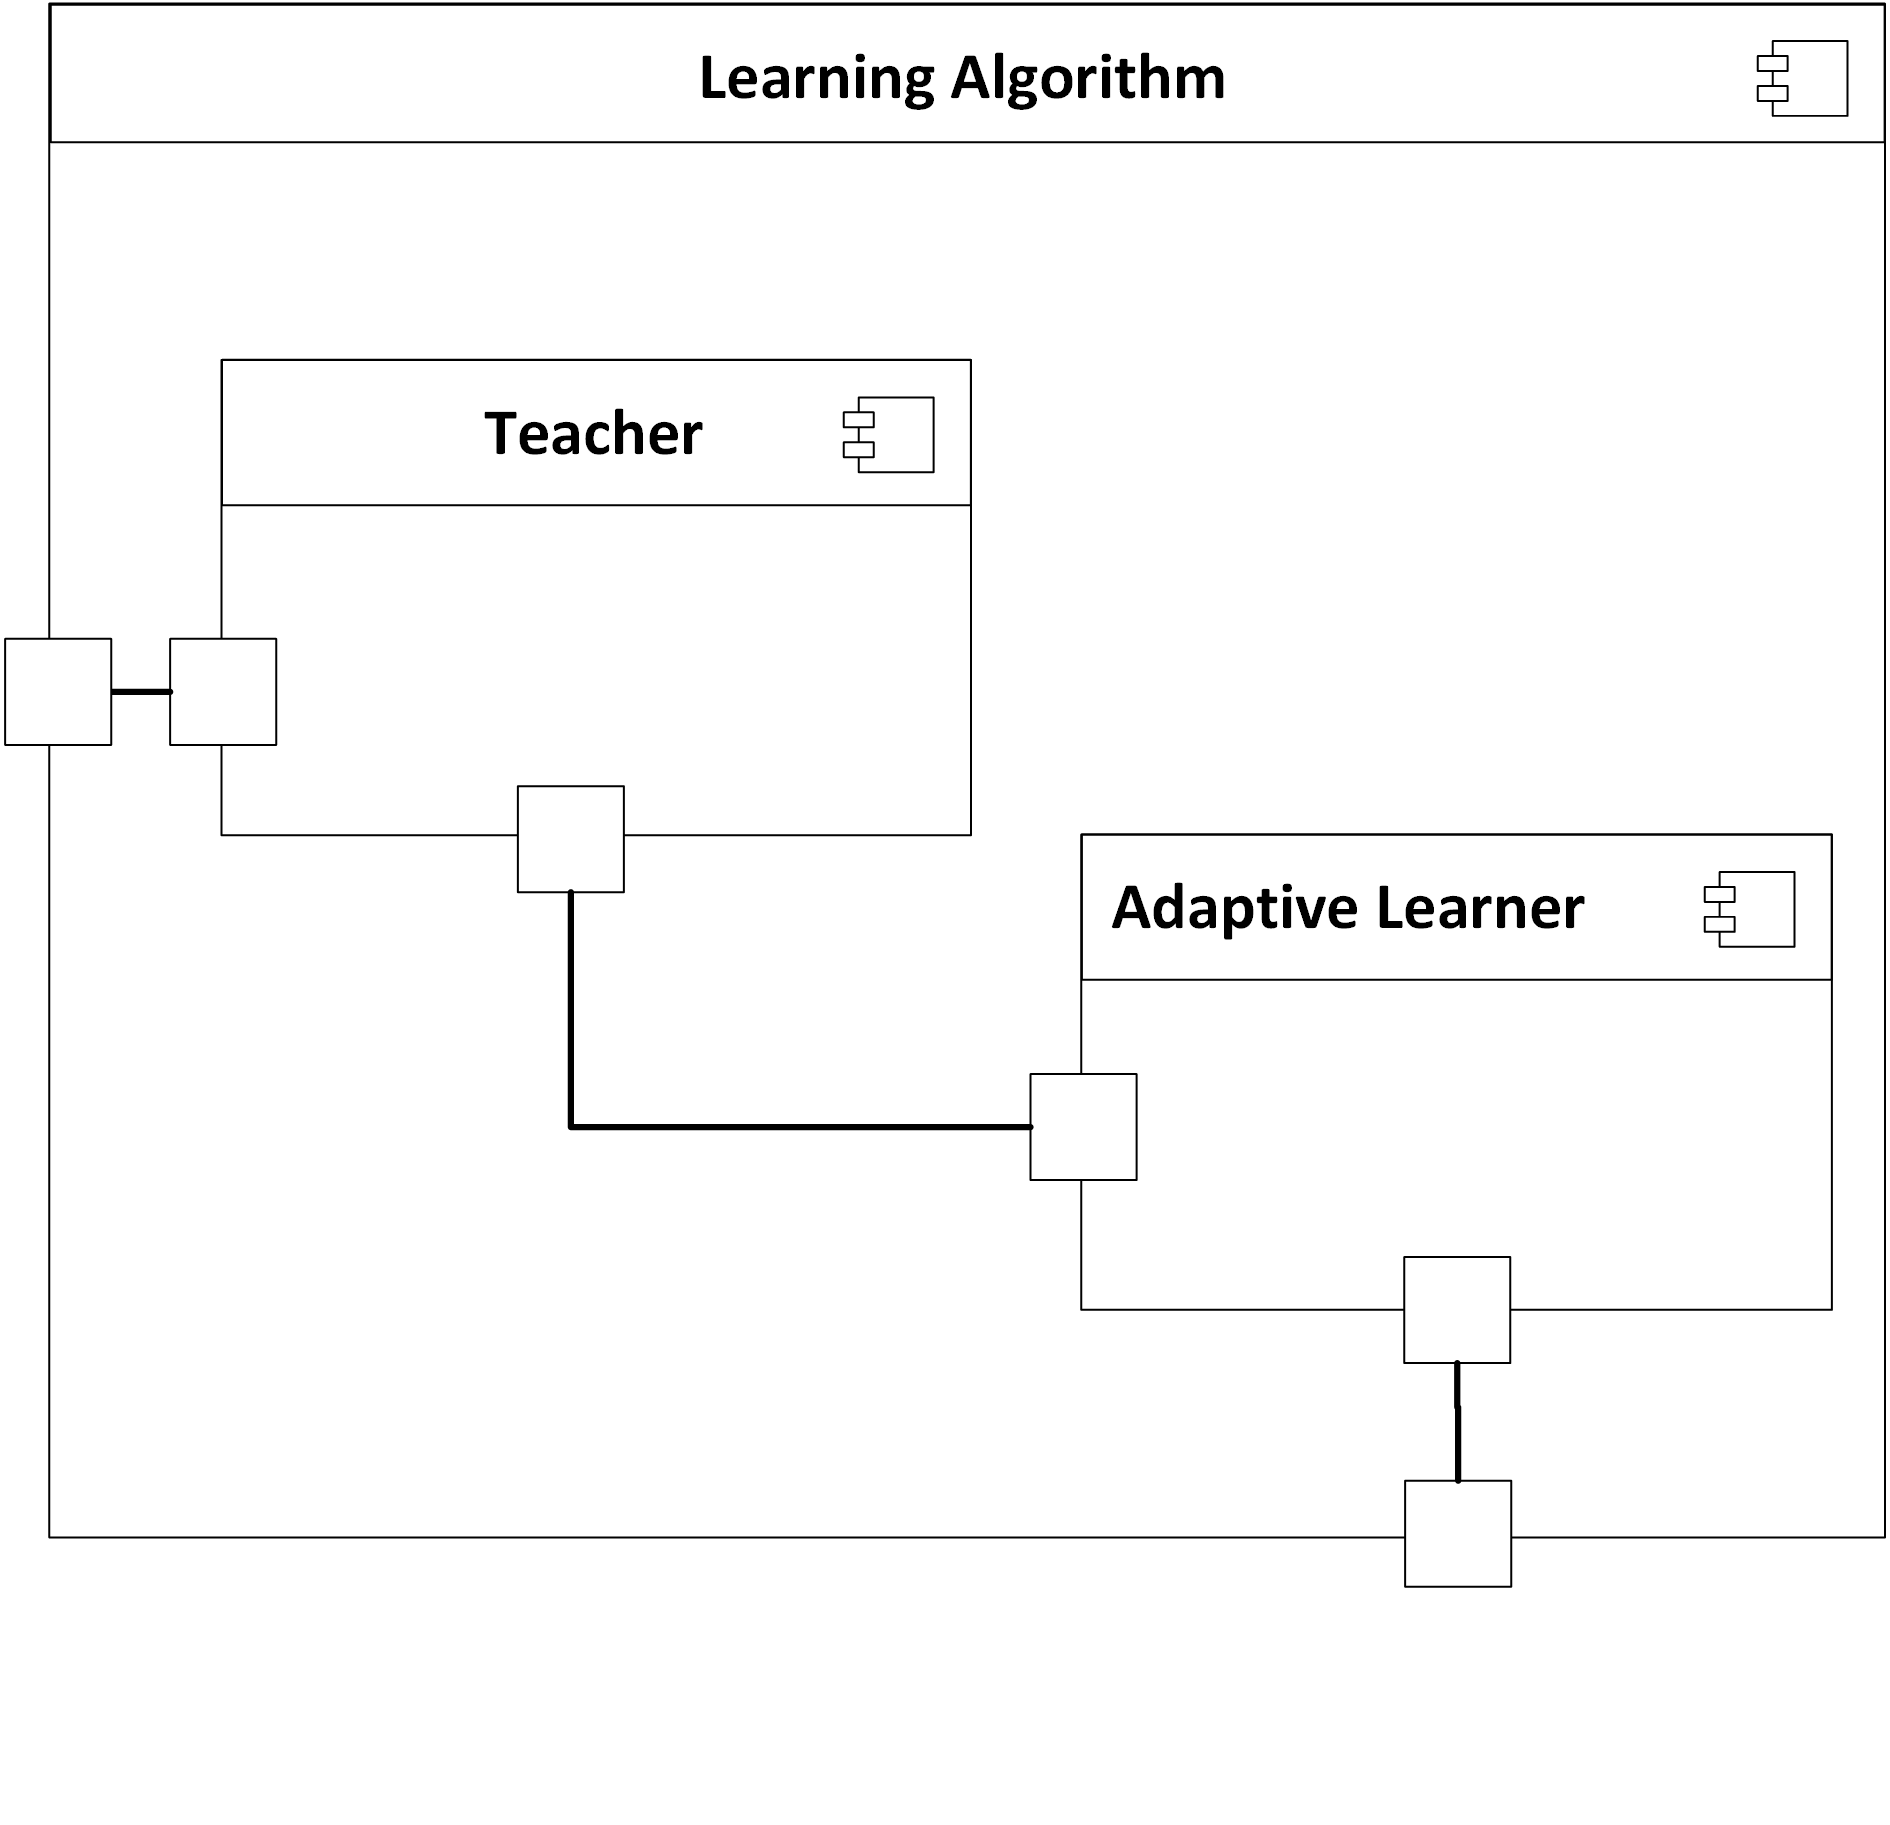
\includegraphics[width=75mm, keepaspectratio]{figures/architecture_learningalgo.png}
	%}
	\caption{Architecture of the Learning Algorithm} 
	\label{fig_architcture_learningalgo}
\end{figure}

\begin{algorithm}[H]
	\SetAlgoLined
	\DontPrintSemicolon
	\KwIn{$S_p$: a set of access sequences, D: a set of suffixes, an input alphabet $\Sigma$}
	\KwOut{A Mealy machine $H=(S, s_0, \Sigma, \Omega, \delta, \lambda)$}
	initialize hypothesis H, create a state for all elements of $S_p$\;
	initialize a queue Q with the states of H\;
	\While{Q is not empty}{
		s = dequeue state from Q\;
		u = access sequence from $s_0$ to s\;
		\For{$d\in D$}{
			output, adaptionCommand = mq($u\*d$)\;
			\If{adaptionCommand is $RESET$}{Go to 1}
			set $\lambda(s,d) = output$\;
		}
		\eIf{exists an $s'\in S$, where the output signature of $s'$ is the same as $s$}{
			reroute transitions of $s$ to $s'$ in H\;
			remove $s$ from H\;
		}{
			\If{adaptionCommand is $OPTIMISTIC$}{create and enqueue successors of $s$ for every input in $\Sigma$ into Q, if not already in $S_p$\;}
		}
	}
	Remove entries of $D\setminus\Sigma$ from $\lambda$\;
	\Return{H}\;
	\caption{Adaptive Direct Hypothesis Construction algorithm}
	\label{algo:adaptivedhc}
\end{algorithm}
%---------------------------------------------------------------
\subsection{Caching} \label{subs_cachingintheframework}
%---------------------------------------------------------------
Caching the previous answers to queries can be a straightforward way of reducing the number of questions the oracle has to answer, specifically in the case of the DHC algorithm, where each learning round makes every single query that the previous did. Thus we introduced a caching layer between the oracle and the learning algorithm, which controls which questions are forwarded to the oracle, and conversely, which can be automatically answered.

In case of the user providing conflicting requirements, as proposed in Subsection \ref{subs_conf}, the user needs to remove one or more requirements, some of which might already have corresponding entries in the cache. Since query responses inferred through some models (such as LTL expressions) are not backwards traceable, there might not be a way to specify exactly which cached entries became outdated. In order to solve this issue, while still enabling the user to provide conflicting requirements, the cache is reset every time a conflict arises, as illustrated on Figure \ref{fig_architcture_ileoverview_cache}. Since the oracle stores the requirements, this does not create extra questions to the user and in most cases can happen in the background through communication of the cache and the oracle. The overview of the resulting framework can be seen in Figure \ref{fig_architcture_informaloverview_complete}.

\begin{figure}[!ht] 
	\centering
	\fbox{
		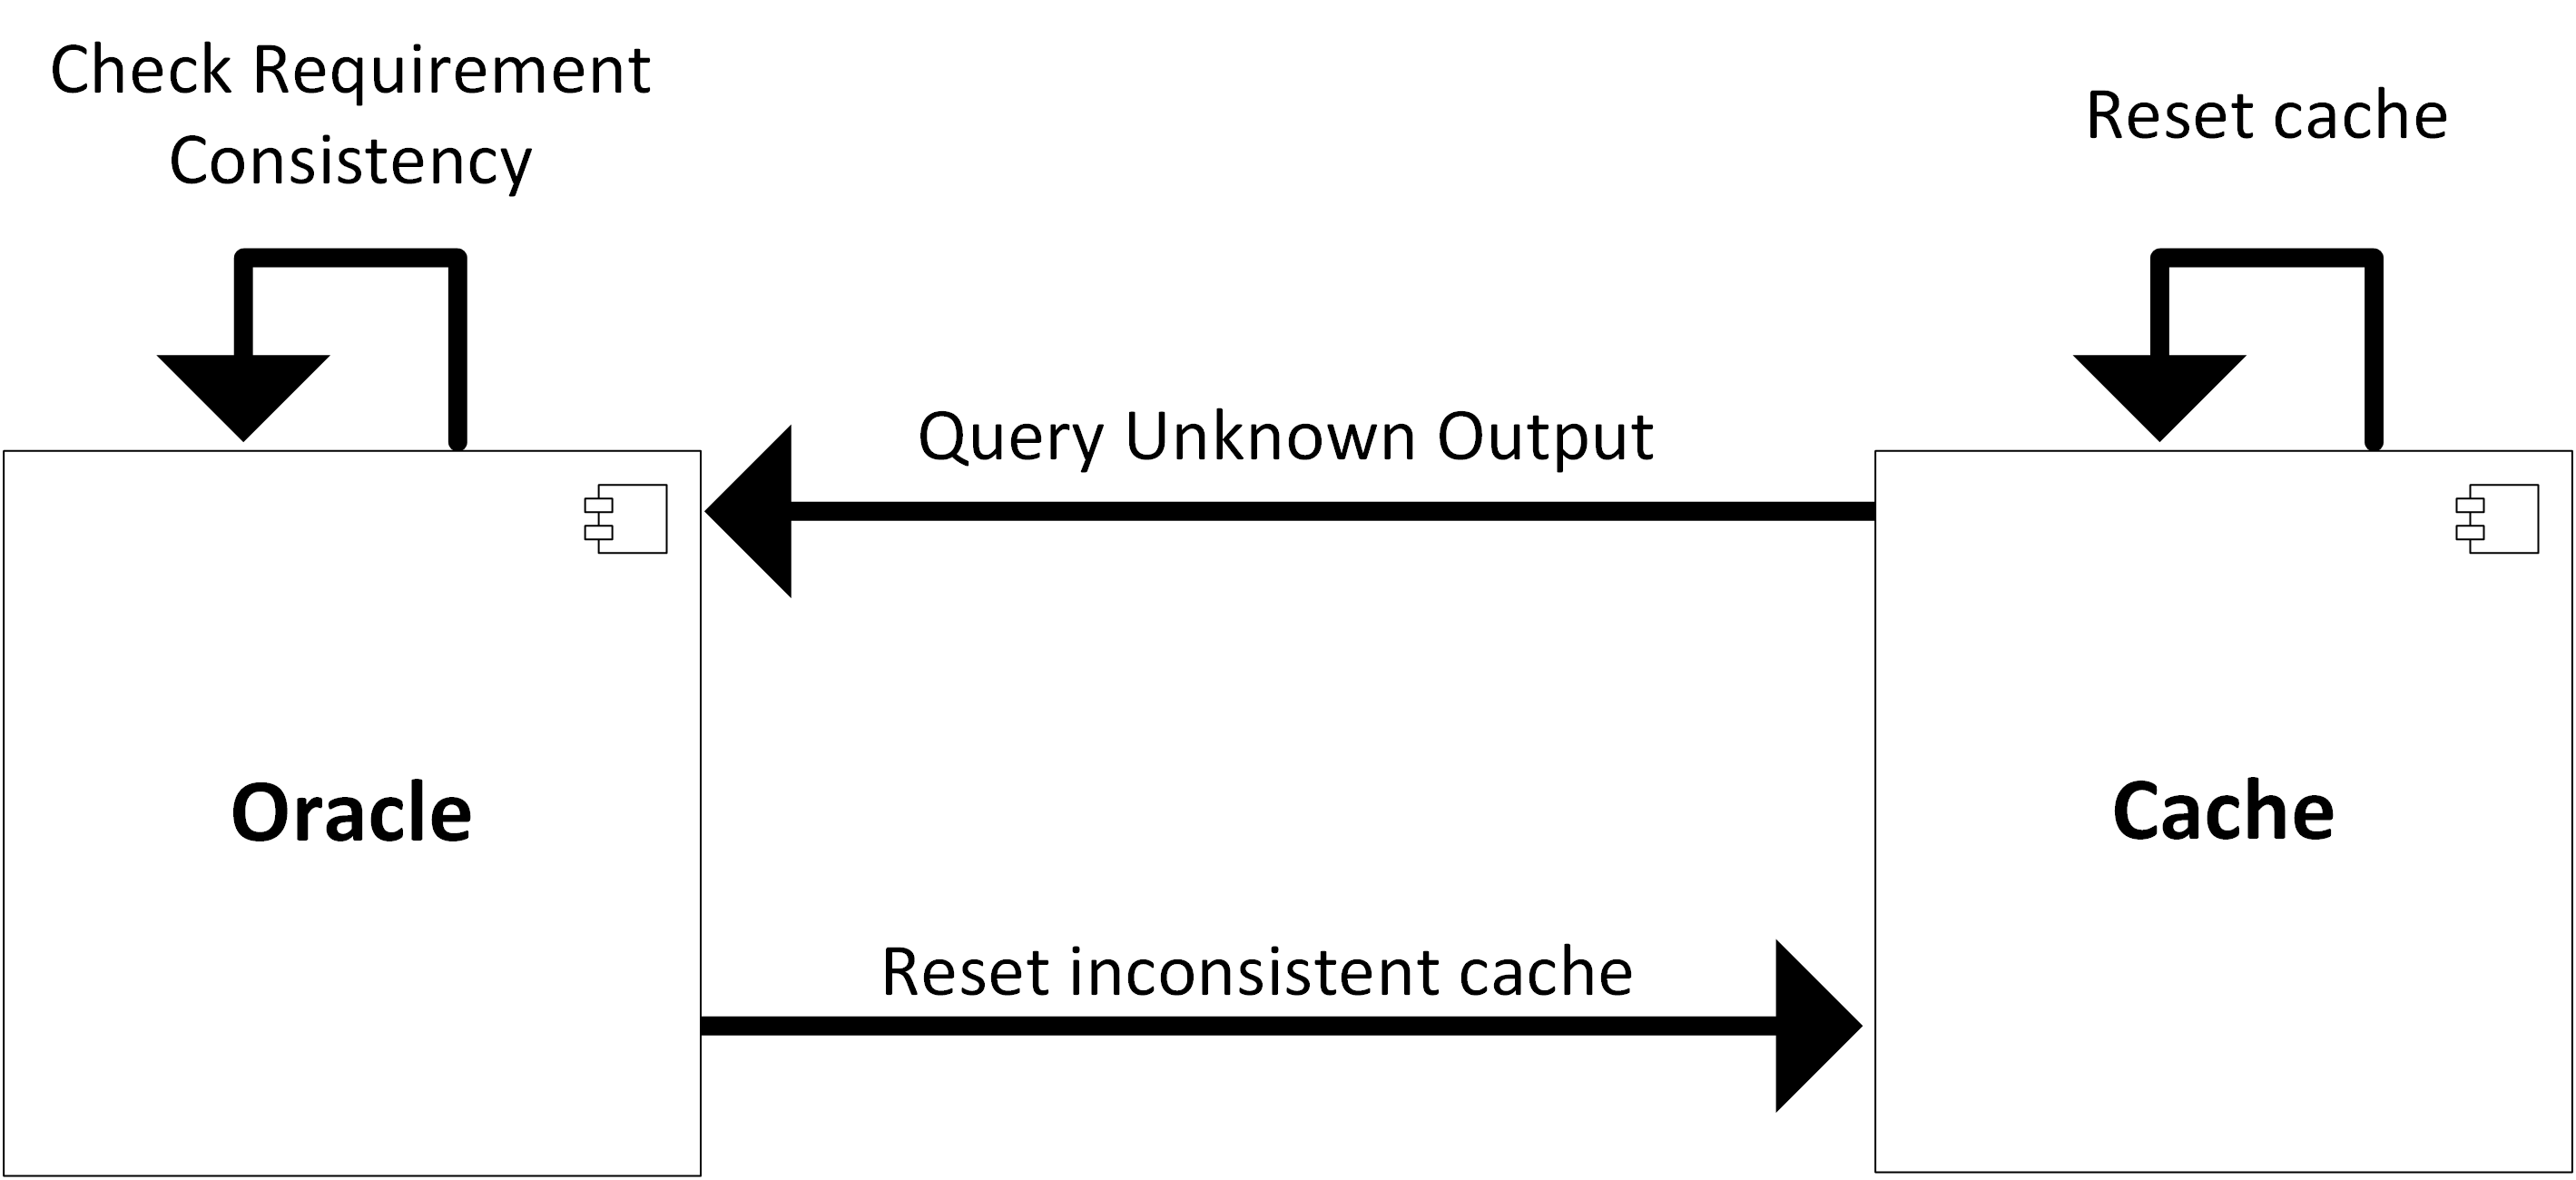
\includegraphics[width=100mm,keepaspectratio]{figures/architecture_informaloverview_cache.png}
	}
	\caption{Overview of cache reset logic} 
	\label{fig_architcture_ileoverview_cache}
\end{figure}



\begin{figure}[!ht] 
	\centering
	\fbox{
		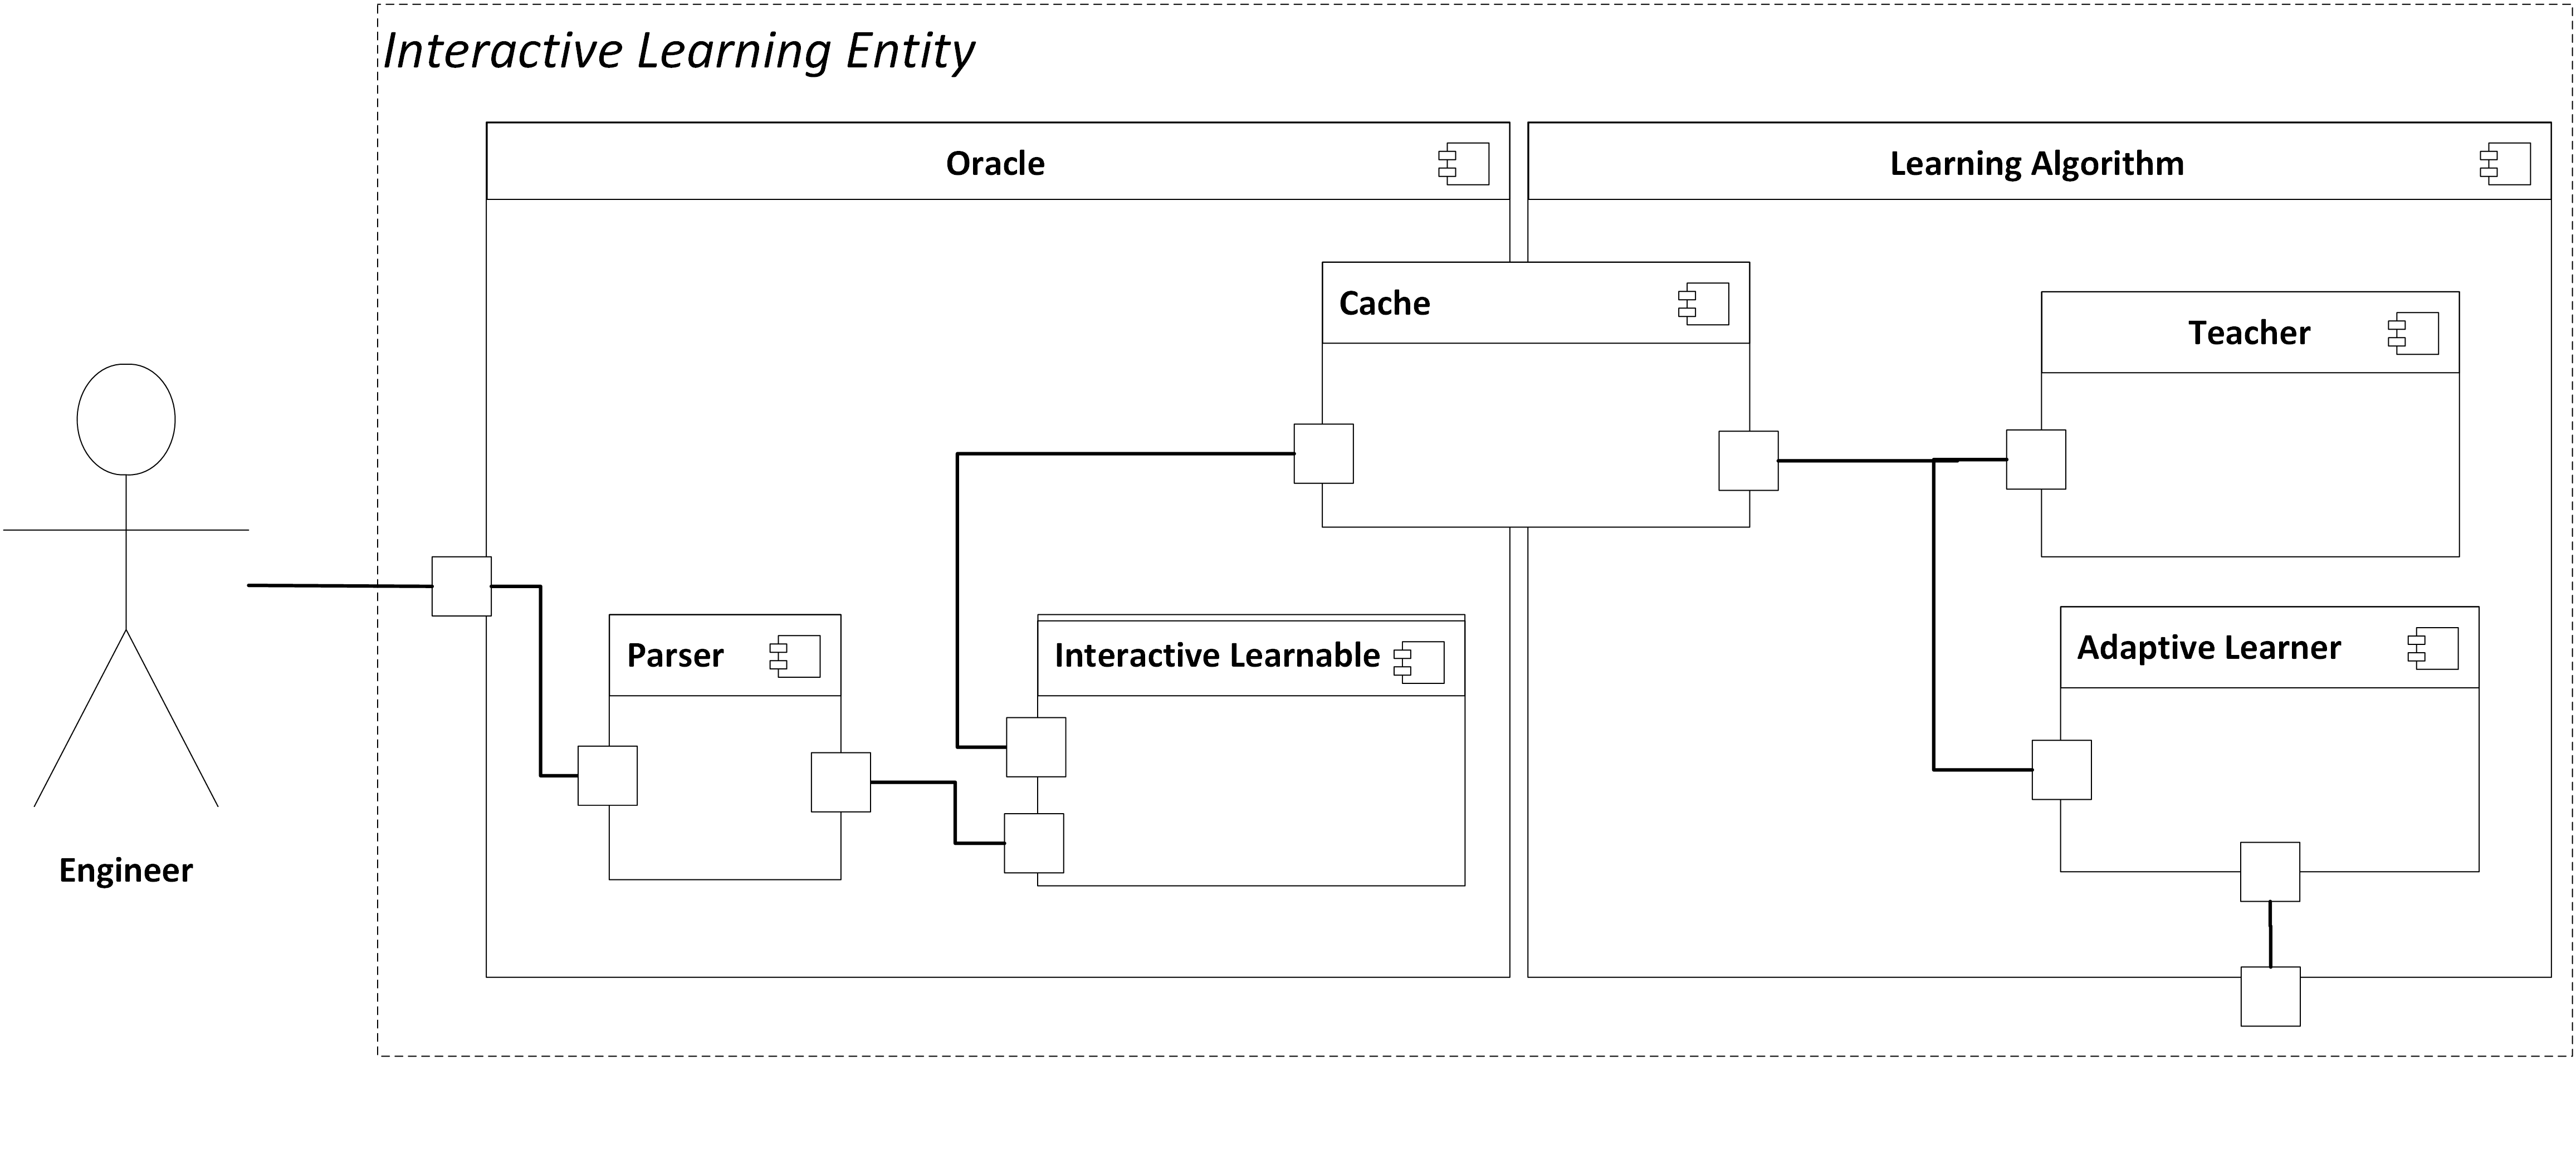
\includegraphics[width=150mm, keepaspectratio]{figures/architecture_informaloverview_complete.png}
	}
	\caption{Architectural overview}
	\label{fig_architcture_informaloverview_complete}
\end{figure}



